\documentclass{article}


\usepackage{appendix}
\usepackage{algorithm,algpseudocode, stmaryrd}
\usepackage[compress]{cite}
\usepackage{afterpage}



% Optional math commands from https://github.com/goodfeli/dlbook_notation.
\newcommand{\bbox}{\text{bbox}}
\newcommand{\alphapck}{\alpha_\bbox}
\newcommand{\kcycle}{\text{k-CyPCK}}
\newcommand{\cycle}{\text{-CyPCK}}

\newcommand{\I}{\mathbf{I}}
\newcommand{\Ia}{\I^\text{a}}
\newcommand{\Ib}{\I^\text{b}}
\newcommand{\Iatob}{\I^\text{a $\rightarrow$ b}}
\newcommand{\F}{\mathbf{F}}
\newcommand{\Fa}{\F^\text{a}}
\newcommand{\Fb}{\F^\text{b}}
\newcommand{\f}{\mathbf{f}}
\newcommand{\fa}{\f^\text{a}}
\newcommand{\fb}{\f^\text{b}}
\newcommand{\p}{\mathbf{p}}
\newcommand{\pa}{\p^\text{a}}
\newcommand{\pb}{\p^\text{b}}
\newcommand{\A}{\boldsymbol{\Phi}_\text{align}}
\newcommand{\G}{\mathbf{G}}
\newcommand{\C}{\mathbf{C}}
\newcommand{\Ca}{\C^\text{a}}
\newcommand{\Cb}{\C^\text{b}}
\newcommand{\cc}{\mathbf{c}}
\newcommand{\cca}{\cc^\text{a}}
\newcommand{\ccb}{\cc^\text{b}}
\newcommand{\Irec}{\I_\text{Recon}}
\newcommand{\M}{\mathbf{M}}
\newcommand{\Mrec}{\M_\text{Recon}}
\newcommand{\loss}{\mathcal{L}}
\newcommand{\T}{\mathcal{T}}
\newcommand{\W}{\mathcal{W}}
\newcommand{\Id}{\mathcal{I}}


\usepackage{hyperref}
\usepackage{url}

\newcommand{\fix}{\marginpar{FIX}}
\newcommand{\new}{\marginpar{NEW}}
\usepackage[left=1in,top=1in,bottom=1in,right=1in]{geometry}

\usepackage{wrapfig}
\usepackage{tikz}
\usetikzlibrary{arrows,decorations.markings}

\tikzset{
  treenode/.style = {shape=rectangle, rounded corners,
                     draw, align=center,
                     top color=white, bottom color=blue!30},
  treenode2/.style = {shape=rectangle, rounded corners,
                     draw, align=center,
                     top color=white, bottom color=green!30},
  env/.style      = {treenode, font=\ttfamily\normalsize},
  env2/.style      = {treenode2, font=\ttfamily\normalsize},
  dummy/.style    = {circle,draw}
}

\usepackage{caption,subcaption}
\usepackage[utf8]{inputenc} % allow utf-8 input
\usepackage[T1]{fontenc}    % use 8-bit T1 fonts
\usepackage{hyperref}       % hyperlinks
\usepackage{url}            % simple URL typesetting
\usepackage{booktabs}       % professional-quality tables
\usepackage{amsfonts}       % blackboard math symbols
\usepackage{nicefrac}       % compact symbols for 1/2, etc.
\usepackage{microtype}      % microtypography
\usepackage{xcolor}         % colors
\usepackage{amsmath, amssymb, amsthm, enumitem}

\newtheorem{theorem}{Theorem}
\newtheorem{lemma}{Lemma}
\newtheorem{definition}{Definition}
\newtheorem{corollary}{Corollary}

\newcommand{\relu}{\phi}

\title{Memorization Capacity of Neural Networks with Conditional Computation}

%On the Fundamental Limits of Conditional Computation in Neural Networks


\author{%
  Erdem Koyuncu \\
  Department of Electrical and Computer Engineering \\
  University of Illinois Chicago\\
  \texttt{ekoyuncu@uic.edu} \\
}

\newcounter{example}[section]
\newenvironment{example}[1][]{\refstepcounter{example}\par\medskip
   \noindent \textbf{Example~\theexample. #1} \rmfamily}{\medskip}



\begin{document}


\maketitle


\begin{abstract}
Many empirical studies have demonstrated the performance benefits of conditional computation in neural networks, including reduced inference time and power consumption. We study the fundamental limits of neural conditional computation from the perspective of memorization capacity. 
For  Rectified Linear Unit (ReLU) networks without conditional computation, it is known that memorizing a collection of $n$ input-output relationships can be accomplished via a neural network with $O(\sqrt{n})$ neurons. Calculating the output of this neural network can be accomplished using $O(\sqrt{n})$ elementary arithmetic operations of additions, multiplications and comparisons for each input. Using a conditional ReLU network, we show that the same task can be accomplished using only $O(\log n)$ operations per input. This represents an almost exponential improvement as compared to networks without conditional computation.\ We also show that the $\Theta(\log n)$ rate is the best possible. Our achievability result utilizes a general methodology to synthesize a conditional network out of an unconditional network in a computationally-efficient manner, bridging the gap between unconditional and conditional architectures. 
\end{abstract}

\section{Introduction}

The increasing complexity of source code poses a key challenge to the reliability of large-scale software systems. Software bugs in these systems can lead to safety issues~\cite{bug_safety} for users around the world as well as cause non-negligible financial losses~\cite{bug_loss}. As such, developers have to spend a large amount of time and effort on bug fixing. Consequently, \aprfull (\apr), designed to automatically generate patches to fix software bugs, has attracted wide attention from both academia and industry~\cite{long2016prophet, legoues2012genprog, long2015spr, lou2020can, tufano2018empstudy}. 


To achieve \apr, one popular approach is known as Generate-and-Validate (G\&V)~\cite{qi2015gv, ghanbari2019prapr, lou2020can, le2016hdrepair, legoues2012genprog, wen2018capgen, hua2018sketchfix, martinez2016astor, koyuncu2020fixminder, liu2019tbar, liu2019avatar}, which is typically based on the following pipeline: First, fault localization techniques~\cite{wong2016fl, abreu2007ochiai, zhang2013injecting, papadakis2015metallaxis, li2019deepfl, li2017transforming} are applied to determine the suspicious locations in programs where bugs are likely to exist. Then, the buggy locations are used by the \apr tools to generate a list of patches that replace buggy lines with correct lines. Afterward, each patch is validated against the original test suite to identify any \emph{plausible patches} (i.e., passing all tests in the test suite). Finally, to determine the \emph{correct patches}, developers examine the list of plausible patches to see if any of them can correctly fix the bug. 

Traditional \apr tools can mainly be categorized into heuristic-based~\cite{legoues2012genprog, le2016hdrepair, wen2018capgen}, constraint-based~\cite{mechtaev2016angelix, le2017s3, demacro2014nopol, long2015spr} and \template~\cite{ghanbari2019prapr, hua2018sketchfix, martinez2016astor, liu2019tbar, liu2019avatar}. Among these traditional tools, \template \apr tools~\cite{ghanbari2019prapr, liu2019tbar, benton2020effectiveness} have been able to achieve state-of-the-art results. \Template \apr tools typically leverage pre-defined templates (e.g., adding a nullness check) for bug fixing. However, since these fix templates are typically handcrafted, the number and types of bugs they are able to fix can be limited. 



To address the limitations of traditional \apr, researchers have proposed various \learning \apr tools~\cite{li2020dlfix, chen2018sequencer, jiang2021cure, lutellier2020coconut, zhu2021recoder, ye2022rewardrepair} based on the \nmtfull (\nmt) architecture~\cite{sutskever2014mt} where the input is the buggy code snippets and the goal is to translate the buggy code snippets into a fixed version. To accomplish this, \learning \apr tools require supervised training datasets with pairs of both buggy and fixed code snippets in order to learn how to perform this translation step. These training data are usually obtained by mining historical bug fixes using heuristics/keywords~\cite{dallmeier2007benchmark}, which can be imprecise for identifying bug-fixing commits; even the actual bug-fixing commits can include irrelevant code changes, leading to further pollution in the dataset~\cite{xia2022alpharepair}.
% 
Moreover, it can be hard for such \apr tools to generalize and fix bug types unseen during training. 



To better leverage recent advances in \plmfull{s} (\plm{s}), researchers~\cite{xia2022alpharepair, xia2023repairstudy, kolak2022patch, prenner2021codexws} have directly applied \plm{s} to generate patches without bug-fixing datasets. These \llm-based \apr tools work by either directly generating a complete code function~\cite{prenner2021codexws, xia2023repairstudy} or predict/infill the correct code snippet given its surrounding context~\cite{xia2022alpharepair, xia2023repairstudy}. By directly using \llm{s} that are pre-trained on billions of open-source code snippets, \llm-based \apr tools can achieve state-of-the-art performance on many repair datasets~\cite{xia2022alpharepair}. 


% 
%
%

Traditional \apr tools have long used the insight of the \emph{plastic surgery hypothesis}~\cite{barr2014plastic} where it states that the code ingredients to fix a bug already exist within the same project. Traditional \apr tools have manually designed pattern-~\cite{ghanbari2019prapr, saha2017elixir} or heuristic-based~\cite{jiang2018simfix, legoues2012genprog} approaches to finding and using such relevant code ingredients to generate fixes for bugs. However, the plastic surgery hypothesis has been largely ignored in \llm-based \apr. In fact, \llm provides a unique opportunity to fully automate the plastic surgery hypothesis idea via fine-tuning (learning project-specific information via model updates from the buggy project) and prompting (directly providing relevant code ingredients to the model), and make it directly applicable to different languages (since the \llm{s} are typically multi-lingual).%
Moreover, despite the intensive manual efforts involved, traditional \apr tools still cannot fully leverage project-specific information due to large search space for leveraging/composing existing code ingredients. In contrast, the project-specific information can effectively leveraged by \llm{s} due to their power in code understanding/vectorization, e.g., even partial/imprecise information may still guide \llm{s} in correct patch generation!
 To this end, we ask the question: \emph{How useful is the plastic surgery hypothesis in the era of \plm{s}}?








\mypara{Our Work.} To answer the question, we present \ourtech{\xspace} -- a \llm-based approach that automatically utilizes the plastic surgery hypothesis by systematically combining multiple fine-tuning and prompting strategies for \apr. \ourtech fine-tunes \plm{s} using two novel domain-specific training strategies: \textbf{\epfinetune} -- we fine-tune using the original buggy project by aggressively masking out a high percentage of tokens, which allows \plm to learn project-specific code tokens and programming styles; and \textbf{\rofinetune} -- which only masks out a single continuous code sequence per training sample, allowing the model to get used to the final \csapr task of predicting a single continuous code sequence. Furthermore, we directly leverage the ability for \plm{s} to understand natural language instructions and introduce a novel prompting strategy, \textbf{\idprompting}, which uses information retrieval and static analysis to obtain a list of relevant identifiers for the buggy lines. While such relevant identifiers are critical for fixing some difficult bugs, they may not be seen by the \llm during inference due to limited context window size. Through the use of prompting, we directly tell the model to use these extracted identifiers (relevant code ingredients) to generate the correct code. Finally, to perform repair, we combine all four model variants (including the base model, both fine-tuned models and the base model with prompting) for the final repair.





While our insight of leveraging the plastic surgery hypothesis for \llm-based \apr is generalizable across different types of \plm{s}, to implement \ourtech, we choose a recent \plm{\xspace}, \ctfive~\cite{wang2021codet5}, which is pre-trained on millions of open-source code snippets. \ctfive is an encoder-decoder model trained using \mspfull (\msp) objective where a percentage of tokens are masked out and each continuous masked token sequence is referred to as a masked span. Also, although we only extract relevant identifiers from the current buggy project (since this paper focuses on the plastic surgery hypothesis), our work can be easily extended to obtain other code information (such as relevant statements or functions) from other sources, such as  the massive pre-training corpora~\cite{husain2020codesearchnet} or historical bug-fixing datasets~\cite{jiang2019infer}, which can provide more coding knowledge for \llm{s}. Besides, although we mainly focus on using traditional string comparison algorithms for information retrieval in this paper, these techniques can be easily replaced by other frequency-based retrieval~\cite{robertson2009probabilistic} and neural search (or embedding-based search)~\cite{reimers2019sentence}.
  In summary, this paper makes the following contributions:


%


\begin{itemize}[noitemsep, leftmargin=*, topsep=0pt]
    \item \textbf{Dimension.} This paper is the first to revisit the important plastic surgery hypothesis in the era of \llm{s}. It opens up a new dimension for \llm-based \apr to incorporate previously neglected information from the buggy project itself to boost \apr performance. Furthermore, it demonstrates the promising future of retrieval-based prompting for modern \llm-based \apr.
    \item \textbf{Implementation.} We implement \ourtech based on the recent \ctfive model. We augment the model using two novel fine-tuning strategies: \epfinetune and \rofinetune, along with a novel prompting strategy based on information retrieval and static analysis: \idprompting. We combine the patches generated by all four models together and perform patch ranking to speed up \apr.% 
    \item \textbf{Evaluation Study.} We conduct an extensive evaluation against state-of-the-art \apr tools. On the widely studied \dfj 1.2 and 2.0 datasets~\cite{just2014dfj}, \ourtech is able to achieve the new state-of-the-art results of 89 and 44 correct bug fixes (15 and 8 more than best baseline) respectively.  Furthermore, we perform a broad ablation study to justify our design. \ourtech demonstrates for the first time that the plastic surgery hypothesis can substantially boost \llm-based \apr and advance state-of-the-art \apr, while being fully automated and general. Moreover, even partial/imprecise code ingredients may still effectively guide \llm{s} for \apr!
\end{itemize}


\section{Proposed Framework: {\ourmodel}}
\label{model}


In this section, we introduce a novel self-supervised co-training framework {\ourmodel}.
The proposed framework is illustrated in Figure~\ref{fig:intro_model} and works in three phases.
Phase one automatically generates two sets of pseudo labels.
We use a combination of off-the-shelf pre-trained POS and NER taggers, knowledge graph, and GPT-2 scorer for generating the first set of pseudo labels automatically without any hand-crafted rules for matching the slot values.
The other set of pseudo labels is acquired through a zero-shot slot filling model~\cite{liu2020coach}, trained on the out-of-domain dataset.
It is critical to emphasize that both sets of labels are noisy and incomplete which poses serious challenges to training effective models for the task of open-domain slot filling.
Phase two fine-tunes the pre-trained BERT to the slot filling task that effectively transfers the knowledge from the pre-trained language model~(LM) to overcome the issue of label incompleteness to some extent. 
Further, we employ the early stopping technique to minimize the noise in the labels.
The output of this phase is two BERT models that can generate soft labels for self-supervision during co-training in phase three.
Phase three leverages the fine-tuned models and further trains them in an iterative fashion.
Specifically, the proposed peer training approach facilitates high-confidence soft label selection for the other peer to perform training. This phase progressively reduces the noise in the labels and enables effective model fitting. 



\subsection{Phase One: Automatic Label Generation}
To acquire the first set of labels, we perform the following steps.
First of all, off-the-shelf trained POS and NER taggers are used to predict initial estimates of the slot values irrespective of the slot types. Then, the type information of the slot values is queried from the KG and the slot value is tagged for the most appropriate slot in the target domain.
This approach, however, produces low recall. 
To expand the candidate slot values, we generate n-grams of the natural language text and employ a partial matching scheme to query the KG for type information (e.g., \myspecial{Jason} \myspecial{Aldean} = \myspecial{American} \myspecial{singer}) of the n-grams if the entry exists.
This process generates multiple overlapping hypotheses about the slot values.
We replace a span of text that corresponds to a slot value by its type information and a GPT-2 based scorer (see Section~\ref{sec:nlpmodels}) is used to select the best candidate based on the fluency of the text.
Naturally, if a token (or span of tokens) is replaced by its type, the sentence should score higher as compared to the case where an inappropriate substitution is performed. 
We select the best hypothesis if the score is greater than the threshold.
Intuitively, the candidate selection threshold can automatically be searched based on a small validation set from the target domain, making the label generation process fully automatic. 
The other set of noisy labels is acquired by the zero-shot slot filling model~\cite{liu2020coach} that has been trained using an out-of-domain dataset. It is important to highlight that the zero-shot slot filling model does not require any labeled in-domain training example. 
To summarize the automatic label generation phase, both sets of labels are acquired in a fully automatic fashion without any hand-crafting.


In contrast to previous work in weak supervision~\cite{ren2015clustype,he2017autoentity,fries2017swellshark,giannakopoulos2017unsupervised} that obtains a single set of noisy labels and then propose techniques to overcome the challenge of fitting an effective model to the noisy labels, we acquire two sets of complementary labels.
The choice of these two sets of labels is guided by the intuition that they should be complementary and the models trained on these sets of labels should be able to share complementary information with the other to improve the performance in the later phases of the framework.
Essentially, the first set of labels carries information from external knowledge sources, whereas the labels generated through the pre-trained zero-shot slot filling model capture how the slot values are mentioned in other domains.
%
To further elaborate on the motivation and our process for the first set of labels (i.e., labels using KG and other NLP models), the pre-trained LMs have been shown to have a great deal of knowledge~\cite{petroni2019language}, thus should be capable of generating automatic labels with no need of external KG. 
To the best of our knowledge, there exists no work that shows that accurate token-level automatic labeling (e.g., slot filling task) is possible with pre-trained LMs. 
Moreover, such approaches would require heavy prompting in each new target domain, whereas our label generation process is fully automatic and only relies on the readily-available pre-trained NLP models and external KG.

\subsection{Phase Two: LM-assisted Weak Supervision}
Since we do not have access to dataset $\{(\mathbf{X}_n,\mathbf{Y}_n)\}_{n=1}^N$ with true ground-truth labels.
We use pseudo labels generated in phase one, $\{(\mathbf{X}_n,\mathbf{D}_n)\}_{n=1}^N$, to learn 
$f_{m,c}(\cdot; \cdot)$ that outputs the probability of the $m$-th token to take on class $c$. 
We learn $f_{m,c}(\cdot; \cdot)$ by minimizing the following loss over the noisy dataset $\{(\mathbf{X}_n,\mathbf{D}_n)\}_{n=1}^N$: 
$$
\hat\theta = \argmin_{\theta}\frac{1}{N}\sum_{n=1}^{N} \ell(\mathbf{D}_n, f(\mathbf{X}_{n}; \theta)),
\label{eq:stage1}
$$
where $\ell(\mathbf{D}_n, f(\mathbf{X}_{n}; \theta)) = \frac{1}{M} \sum_{m=1}^{M} -\log{f_{m,d_{n, m}}(\mathbf{X}_{n}; \theta)}$. 
We employ the pre-trained multilingual BERT with token-level classification head that uses Adam optimizer \cite{kingma2014adam,Liu2019} with early stopping and multiple random initializations. 


Since slot filling task is similar to the MLM training objective of the BERT, we employ pre-trained BERT as the backbone model.
That is, MLM's goal is to predict the masked tokens using bidirectional contexts. Similarly, slot filling tries to predict the label for a token leveraging both left and right contexts simultaneously, which makes the pre-trained BERT an ideal model of choice that greatly facilitates minimizing incomplete labels.
It is important to highlight that our automatically generated labels are not only incomplete but also potentially wrong.
The training strategies employed in this phase minimize the noise in the label to some extent. 
Specifically, early stopping can provide a strong regularization and would not let the model overfit to the noisy labels, especially wrong labels. 
Moreover, early stopping does not let the model forget the knowledge in the pre-trained model.
Similarly, multiple random initializations enforce robustness. 
Since the model is fine-tuned on the noisy labels, averaging the predictions of multiple models for each token ensures that wrong labels end up with low probabilities and true labels consistently achieve high probabilities.
Using the above-mentioned strategies, we train two slot filling models, which we call the peers. The peer one is trained on the first set of pseudo labels that were generated using POS and NER taggers, KG, and the GPT-2 scorer in phase one. Similarly, peer two is trained using the predictions of the zero-shot slot filling model~\cite{liu2020coach}.
Both models have the same architecture and follow the same training procedures.

\begin{table*}[t!]
\centering
\caption{Dataset statistics.}
\vspace{-7pt}
\label{tab:dataset}
\begin{tabular}{lccccc}
\toprule
\textbf{Dataset}  & \textbf{Dataset Size} & \textbf{Vocab. Size} & \textbf{Avg. Length} & \textbf{\# of Domains} & \textbf{\# of Slots} \\ \hline
\textbf{SGD}      & 188K                  & 33.6K                & 13.8                 & 20                     & 240                  \\
\textbf{MultiWoZ} & 67.4K                 & 10.5K                & 13.3                 & 8                      & 61 \\
\bottomrule
\end{tabular}
\vspace{-7pt}
\end{table*}

\subsection{Phase Three: Self-supervised Co-training}
We introduce an iterative peer training algorithm where both peers generate high-confidence soft labels for training the other peer in the next iteration. 
Theoretically, these peers can be anything, but in this work, 
we explore two of the most promising directions that have shown the promise to minimize the need for manual labeling for the task: zero-shot learning and distant supervision.
This phase uses a self-supervised co-training scheme to exploit the patterns of slot values from other domains through the labels generated by the zero-shot filling model (i.e., peer two)~\cite{liu2020coach} as well as utilize the knowledge in external KGs and pre-trained models via labels provided by the peer one.
Specifically, we initialize the peers trained in phase two and use their pseudo labels to kick-start training in this phase.
Specifically, peer one $f_{m,c}(\cdot; \theta_{\textrm{p1}})$ would generate labels $\{\tilde{\mathbf{Y}}^{(t)}_n = [\tilde{y}_{n,1}^{(t)}, ..., \tilde{y}_{n,m}^{(t)}]\}_{n=1}^{N}$ for peer two $f_{m,c}(\cdot; \theta_{\textrm{p2}})$ at the $t$-th iteration by:
$$
\tilde{y}_{n,m}^{(t)} = \argmax_{c}{f_{m,c}(\mathbf{X}_n; \theta_{\textrm{p1}}^{(t)})}. 
\label{eq:pseudo}
$$

Based on these labels, the peer two can be fine-tuned by: 
$$
\hat\theta_{\textrm{p2}}^{(t+1)} = \argmin_{\theta}\frac{1}{N}\sum_{n=1}^N \ell(\tilde{\mathbf{Y}}_n^{(t)}, f(\mathbf{X}_{n}; \theta)).
\label{eq:self_train1}
$$

Similarly, peer two $f_{m,c}(\cdot; \theta_{\textrm{p2}})$ would generate pseudo labels for peer one $f_{m,c}(\cdot; \theta_{\textrm{p1}})$ that are used to fine-tune peer one. 
We also notice that it is beneficial to stop early during this phase as well, to improve the model fitting and gradually reduce the noise associated with the automatically generated labels.
Since pseudo labels are refined gradually in an iterative way, both peers can benefit from the knowledge contained within the labels of the other while avoiding overfitting.
Furthermore, as an alternative to pseudo labels, we also generate soft labels that are used for confidence re-weighting. 
The high-confidence soft label selection strategy enables better model fitting and efficient learning via better quality of the automatic labels.
Specifically, for the given $m$-th token in the $n$-th training example, the probability for all classes $C$ is $[f_{m,1}(\mathbf{X}_n;\theta),...,f_{m,C}(\mathbf{X}_n;\theta)]$. 
Following ~\cite{xie2016unsupervised}, at $t$-th iteration, peer one generates soft labels, $\{\mathbf{S}_n^{(t)} = [\mathbf{s}_{n,m}^{(t)}]_{m=1}^M \}_{n=1}^N$, as given below:
$$
\mathbf{s}_{n,m}^{(t)} = [s_{n,m,c}^{(t)}]_{c=1}^{C} = \Bigg[  \frac{f_{m,c}^2(\mathbf{X}_n;\theta_{\textrm{peer1}}^{(t)})/p_{c}}{\sum_{c'=1}^C f_{m,c'}^2(\mathbf{X}_n;\theta_{\textrm{peer1}}^{(t)})/p_{c'}}\Bigg]_{c=1}^{C}
\label{eq:soft}
$$ 
where $p_{c} = \sum_{n=1}^N \sum_{m=1}^M f_{m,c}(\mathbf{X}_n;\theta_{\textrm{p1}}^{(t)})$ computes the frequency of the tokens for the $c$-th class. 
Then, peer two $f(\cdot; \theta_{\textrm{p2}}^{(t+1)})$ is fine-tuned by:
$$
\theta_{\textrm{p2}}^{(t+1)} = \argmin_{\theta} \frac{1}{N} \sum_{n=1}^{N} \ell_{\rm KL}(\mathbf{S}_n^{(t)}, f(\mathbf{X}_{n}; \theta)),
$$
where $\ell_{\rm KL}(\cdot,\cdot)$ is the KL-divergence-based loss:
$$
\ell_{\rm KL}(\mathbf{S}_n^{(t)}, f(\mathbf{X}_{n}; \theta))=\frac{1}{M}\sum_{m=1}^M\sum_{c=1}^C - s_{n,m,c}^{(t)} \log f_{m,c}(\mathbf{X}_{n}; \theta).
\label{eq:klloss}
$$

Moreover, we also investigate selecting tokens that have high confidence. 
For instance, we pick high-confidence tokens from the $m$-th input example at the $t$-th iteration by  
$
H^{(t)}_n = \{m : \max_{c} s_{n,m,c}^{(t)} > \epsilon \},
$
where $\epsilon\in [0,1]$ is a threshold that can be searched based on a small validation set. 
Then, peer two $f(\cdot; \theta_{\textrm{p2}}^{(t+1)})$ is fine-tuned by:
$$
\theta_{\textrm{p2}}^{(t+1)} %&= \argmin_{\theta} \frac{1}{N} \sum_{n=1}^{N} \ell_{\rm S-KL}(\bS_n^{(t)}, f(\bX_{n}; \theta)) \\
= \argmin_{\theta} \frac{1}{N|H^{(t)}_n|}\sum_{n=1}^{N} \sum_{m\in H^{(t)}_n}\sum_{c=1}^C - s_{n,m,c}^{(t)} \log f_{m,c}(\mathbf{X}_{n}; \theta).
$$

This phase improves the robustness to effectively fit the model for tokens with high confidence. 
Both peers keep sharing information and their confidence by producing soft labels for their counterparts until they approximate to the true labels while employing early stopping and scheduled learning rates.
It is important to remind that phase three is the most important phase that progressively reduces noise from the labels to a great extent and enables superior performance for the task of open-domain slot filling.
\section{Memorization with Low Computational Complexity}
\label{sec:reluach}

In this section, we introduce our ReLU network to memorize the input-output relationships $x_i \mapsto d_i,\,i=1,\ldots,n$. Our network will only yield $O(\log n)$ active neurons and weights per input. Application of Theorem \ref{th:synth} will then imply a conditional network that can achieve perfect recall with only $O(\log n)$ operations per input, as desired.

 Given a neural network $f$, and  an input $x$ to $f$, let $A(x;f)$ and $W(x;f)$ denote the number of active neurons and active weights, respectively. Our feedforward ReLU network construction is provided by the following theorem.
\begin{theorem}
\label{th:reluach}
Let $X = \{x_1,\ldots,x_n\}\subset\mathbb{R}^p$ be a dataset of input patterns such that for every $i,j\in\{1,\ldots,n\}$ with $i\neq j$, we have $x_i \neq x_j$. Let $\bar{x}_i = [\begin{smallmatrix} 1 \\ x_i \end{smallmatrix}]\in\mathbb{R}^{q}$, where $q=1+p$, be the augmented dataset patterns for biasing purposes. Let $d_1,\ldots,d_n\in\mathbb{R}^r$ be the corresponding desired outputs. Suppose every component of $d_i$ is non-negative for each $i\in\{1,\ldots,n\}$. Then, there is a neural network $f:\mathbb{R}^{q}\rightarrow\mathbb{R}^r$ such that for every $i\in\{1,\ldots,n\}$, we have $f(\bar{x}_i) = d_i$, 
\begin{align}
\label{eq:th1actneuronbound} 	A(\bar{x}_i;f) & \leq 2(q+1)\lceil \log_2 n \rceil + q+r \in O(r+q\log n), \\
%\end{align}
%and
%\begin{align}
\label{eq:th1actweightbound} 	W(\bar{x}_i;f)  & \leq 12q(q+1)\lceil \log_2 n \rceil + (r+2)q+r-2  \in O(rq+q^2\log n).
\end{align}



%\begin{align}
%\nonumber 
%A(\bar{x}_i;f) & \leq (q+r+2)\lceil \log_2 n \rceil + q+r-1 \\
%\label{eq:th1actneuronbound} & \in O((q+r)\log n).
%\end{align}
%Moreover, every neuron in network $f$ has at most $q$ incoming weights, resulting in $O(q(q+r)\log n)$ active weights per input according to (\ref{eq:th1actneuronbound}).


%the following statements hold.
%\begin{enumerate}[label={[\roman*]}]
%\item There is a neural network $f:\mathbb{R}^{q}\rightarrow\mathbb{R}^r$ and a constant $C_1\in\mathbb{R}$ such that $A(\bar{x}_i;f) \leq \log_2 n + C_1$ and $f(\bar{x}_i) = d_i,\,\forall i\in\{1,\ldots,n\}$.
%\item There is a neural network $f:\mathbb{R}^{q}\rightarrow\mathbb{R}^r$ and a constant $C_2\in\mathbb{R}$ such that $A(\bar{x}_i;f) \leq 2\log_2 n + C_2$ and $f(\bar{x}_i) = d_i,\,\forall i\in\{1,\ldots,n\}$. Each neuron in the network has in-degree at most $q=1+p$.
%\end{enumerate}
\end{theorem}
\begin{proof} (Sketch)
We provide an illustrative sketch of the proof. Suppose we wish to memorize the two-dimensional dataset given by Fig. \ref{fig:divideandconquera}. We can divide the datasets to two parts via a line, the resulting two parts to further two sub-parts, and so on, until reaching singletons, as shown in Fig. \ref{fig:divideandconquerb}. The overall network architecture that achieves the performance in the statement of the theorem is then shown in Fig. \ref{fig:nnforachievability}. The initial block $\mathbf{T}$ is a basic preprocessing translation. The ``switch'' $\mathbf{S}_{ij}$ corresponds to the line parameterized by weights $w_{ij}$ in Fig. \ref{fig:divideandconquerb}. The switch $\mathbf{S}_{ij}$ routes the zero vector to one output path and copy its input to the other output path, depending on the side of the $w_{ij}$-line its input vector resides. The switches are followed by ReLU neurons with weights $\gamma_i$. These neurons  map the corresponding input pattern on the active path to its desired output. Finally, the output of the $\gamma_i$-neurons are accumulated. As an example, the signals on the graph for input pattern $\bar{x}_6$ is provided, with $\bar{\bar{x}}_6 \triangleq \mathbf{T}(\bar{x}_6)$. In general, all input-output relationships are satisfied with $O(\log n)$ active neurons per dataset sample. We refer to the complete proof in Appendix \ref{sec:reluachthproofer} for the precise bounds.
\end{proof}

\begin{corollary}
	\label{toyotacorolla}
	Let $x_i,d_i,\,i=1,\ldots,n$ be a sequence of arbitrary input-output pairs as stated in Theorem \ref{th:reluach}. Then, there is a conditional network that, for every $i$, provides an output of $d_i$ whenever the input is $x_i$ by performing only $O(rq+q^2\log n)$ operations.
\end{corollary}
\begin{proof}
We apply the synthesis procedure in Theorem \ref{th:synth} to the network constructed in Theorem \ref{th:reluach}. An alternative more ``direct'' proof (that does not need Theorem \ref{th:synth}) is to implement the gating blocks $\mathbf{S}_{ij}$ in Fig. \ref{fig:divideandconquer} via if-else conditioning statements, resulting in a similar architecture.
\end{proof}



We recall that for ReLU networks without conditional computation, the best achievability result \cite{vardi2021optimal} requires $O(\sqrt{n\log n})$ neurons and weights for memorizing a dataset of size $n$. Since the construction in \cite{vardi2021optimal} is not optimized for conditional computation, it is easily observed that every input activates all $O(\sqrt{n\log n})$ neurons and weights of the network, resulting in $O(\sqrt{n \log n})$ active weights per input. In fact, the remarkable construction in \cite{vardi2021optimal} is a narrow network of a finite width of only $12$, but depth $O(\sqrt{n\log n})$. Even if every input activates only one neuron at each layer, one obtains $O(\sqrt{n\log n})$ active neurons or arithmetic operations per input. In contrast, we only need $O(\log n)$ active weights or operations (via Corollary \ref{toyotacorolla}) per input.


The fact that one cannot fundamentally achieve a sub-polynomial number of neurons without conditional computation is an easy consequence of the VC dimension theory. In our setting, the VC dimension corresponds to the cardinality of the largest dataset that can be memorized. Hence, upper bounds on the VC dimension translate to lower bounds on the memorization capacity. In this context, \cite[Theorem 8.6]{anthony1999neural} provides an $O(n_w^2)$ upper bound on the VC dimension for ReLU networks, where $n_w$ denotes the number of weights in the network. Since any upper bound on the VC dimension is also an upper bound on the cardinality of the largest possible dataset that can be memorized, we have $n \in O(n_w^2)$. It follows that $n_w \in \Omega(\sqrt{n})$ weights are the best possible for ReLU networks without conditional computation, meaning that the results of \cite{vardi2021optimal} are optimal up to logarithmic factors. Also, using the bound $n_w \leq n_e^2$, where $n_e$ is the number of neurons in the network (equality holds in the extreme scenario where every neuron is connected to every other neuron, including itself), we obtain the necessity of $\Omega(n^{1/4})$ neurons. 


\begin{figure}[h]\centerline{
     \begin{subfigure}[b]{0.45\textwidth}
\centerline{\scalebox{0.85}{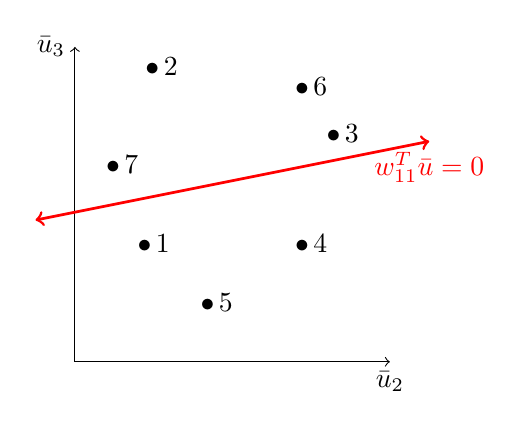
\begin{tikzpicture}

\draw[->] (0,0) -- (4,0) node[anchor=north] {$\bar{u}_2$};
\draw[->] (0,0) -- (0,4) node[anchor=east] {$\bar{u}_3$};
\draw (1,1.5) node {$\bullet\,1$}; %label
\draw (0.6,2.5) node {$\bullet\,7$}; %label
\draw (1.8,0.75) node {$\bullet\,5$}; %label
\draw (1.1,3.75) node {$\bullet\,2$}; %label
\draw (3.4,2.9) node {$\bullet\,3$}; %label
\draw (3,1.5) node {$\bullet\,4$}; %label
\draw (3,3.5) node {$\bullet\,6$}; %label
\draw[line width=1pt, red, <->] (-0.5,1.8) -- (4.5,2.8) node[anchor=north] {$w_{11}^T\bar{u} = 0$};
\end{tikzpicture}}}
\vspace{-5pt}
\caption{Dividing a set of point to two equal subsets.}
\label{fig:divideandconquera}
\end{subfigure}
     \begin{subfigure}[b]{0.45\textwidth}
\centerline{\scalebox{0.85}{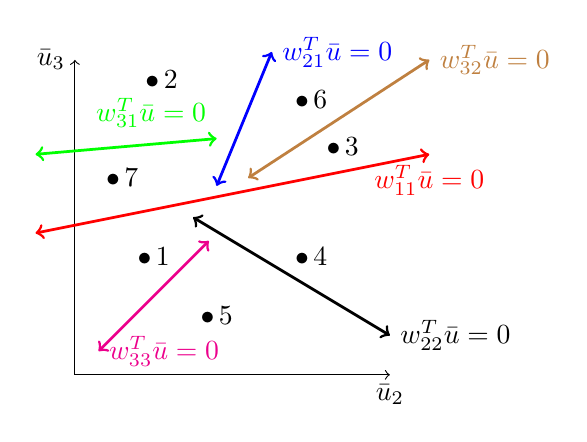
\begin{tikzpicture}

\draw[->] (0,0) -- (4,0) node[anchor=north] {$\bar{u}_2$};
\draw[->] (0,0) -- (0,4) node[anchor=east] {$\bar{u}_3$};
\draw (1,1.5) node {$\bullet\,1$}; %label
\draw (0.6,2.5) node {$\bullet\,7$}; %label
\draw (1.8,0.75) node {$\bullet\,5$}; %label
\draw (1.1,3.75) node {$\bullet\,2$}; %label
\draw (3.4,2.9) node {$\bullet\,3$}; %label
\draw (3,1.5) node {$\bullet\,4$}; %label
\draw (3,3.5) node {$\bullet\,6$}; %label
\draw[line width=1pt, red, <->] (-0.5,1.8) -- (4.5,2.8) node[anchor=north] {$w_{11}^T\bar{u} = 0$};
\draw[line width=1pt, blue, <->] (1.8,2.4) -- (2.5,4.1) node[anchor=west] {$w_{21}^T\bar{u} = 0$};
\draw[line width=1pt, brown, <->] (2.2,2.5) -- (4.5,4) node[anchor=west] {$w_{32}^T\bar{u} = 0$};
\draw[line width=1pt, black, <->] (1.5,2) -- (4,0.5) node[anchor=west] {$w_{22}^T\bar{u} = 0$};
\draw[line width=1pt, magenta, <->] (1.7,1.7) -- (0.3,0.3) node[anchor=west] {$w_{33}^T\bar{u} = 0$};
\draw[line width=1pt, green, <->] (-0.5,2.8) -- (1.8,3) node[anchor=south east] {$w_{31}^T\bar{u} = 0$};
\end{tikzpicture}}}
\vspace{-5pt}
\caption{Continued divisions until reaching singletons.}
\label{fig:divideandconquerb}
\end{subfigure}}
\vspace{-5pt}
\caption{The divide and conquer strategy.}
\label{fig:divideandconquer}
\end{figure}


%\begin{figure}
%\centerline{\begin{tikzpicture}[
%arrowstyle/.style={decoration={markings,mark=at position 1 with
%    {\arrow[scale=1.7,>=stealth]{>}}},postaction={decorate}},
%roundnode/.style={circle, draw=blue!60, fill=blue!5, very thick, minimum size=2mm},
%squarednode/.style={rectangle, draw=green!60, fill=yellow!5, very thick, minimum size=5mm},
%squarednode2/.style={rectangle, draw=magenta!60, fill=magenta!5, very thick, minimum size=5mm},
%squarednode3/.style={rectangle, draw=blue!60, fill=blue!5, very thick, minimum size=5mm},
%squarednode4/.style={rectangle, draw=red!60, fill=red!5, very thick, minimum size=5mm},]
%
%\node[inner sep=0pt, minimum size=3mm](n1x) at (-0.75,-0.5){$=[\begin{smallmatrix} 1 \\ x_6 \end{smallmatrix}]$};
%
%\node[inner sep=0pt, minimum size=3mm](n1) at (-1,0) {$u=\bar{x}_6$};
%\node[squarednode](t) at (0.5,0) {$\mathbf{T}$};
%\draw [arrowstyle](n1)--(t);
%\node[squarednode2](s11) at (2.5,0) {$\mathbf{S}_{11}$};
%\draw [arrowstyle](t)--node [below] {$\bar{u}=\bar{\bar{x}}_6$}(s11);
%\node[squarednode2](s21) at (4,1.8) {$\mathbf{S}_{21}$};
%\node[squarednode2](s22) at (4,-1.8) {$\mathbf{S}_{22}$};
%\draw [arrowstyle](s11)--node [below] {$\,\,\bar{\bar{x}}_6$}(s21);
%\draw [arrowstyle](s11)--node [below] {$0$}(s22);
%\node[squarednode2](s32) at (5.5,0.9) {$\mathbf{S}_{32}$};
%\node[squarednode2](s31) at (5.5,2.7) {$\mathbf{S}_{31}$};
%\node[squarednode2](s33) at (5.5,-2.7) {$\mathbf{S}_{33}$};
%
%\draw [arrowstyle](s21)--node [below] {$0$}(s31);
%\draw [arrowstyle](s21)--node [below] {$\!\!\bar{\bar{x}}_6$}(s32);
%\draw [arrowstyle](s22)--node [below] {$0$}(s33);
%
%\node[squarednode3](g2) at (7,3.15) {$\gamma_2^T$};
%\node[squarednode3](g2r) at (8,3.15) {$\relu$};
%
%\node[squarednode3](g7) at (7,2.25) {$\gamma_7^T$};
%\node[squarednode3](g7r) at (8,2.25) {$\relu$};
%
%\node[squarednode3](g6) at (7,1.35) {$\gamma_6^T$};
%\node[squarednode3](g6r) at (8,1.35) {$\relu$};
%
%\node[squarednode3](g3) at (7,0.45) {$\gamma_3^T$};
%\node[squarednode3](g3r) at (8,0.45) {$\relu$};
%
%\node[squarednode3](g5) at (7,-3.15) {$\gamma_5^T$};
%\node[squarednode3](g5r) at (8,-3.15) {$\relu$};
%
%\node[squarednode3](g1) at (7,-2.25) {$\gamma_1^T$};
%\node[squarednode3](g1r) at (8,-2.25) {$\relu$};
%
%\node[squarednode3](g4) at (7,-0.9) {$\gamma_4^T$};
%\node[squarednode3](g4r) at (8,-0.9) {$\relu$};
%
%\draw [arrowstyle](s31)--node [above] {$0$}(g2);
%\draw [arrowstyle](s31)--node [below] {$0$}(g7);
%\draw [arrowstyle](s32)--node [above] {$\bar{\bar{x}}_6$}(g6);
%\draw [arrowstyle](s32)--node [below] {$0$}(g3);
%\draw [arrowstyle](s22)--node [above] {$0$}(g4);
%\draw [arrowstyle](s33)--node [above] {$0$}(g1);
%\draw [arrowstyle](s33)--node [below] {$0$}(g5);
%
%\draw [arrowstyle](g1)--(g1r);
%\draw [arrowstyle](g2)--(g2r);
%\draw [arrowstyle](g3)--(g3r);
%\draw [arrowstyle](g4)--(g4r);
%\draw [arrowstyle](g5)--(g5r);
%\draw [arrowstyle](g6)--(g6r);
%\draw [arrowstyle](g7)--(g7r);
%
%
%\node[squarednode4](sumnode) at (10,0) {$\sum$};
%\draw [arrowstyle](g1r)--node [above] {$0$}(sumnode); 
%\draw [arrowstyle](g2r)--node [above] {$0$}(sumnode); 
%\draw [arrowstyle](g3r)--node [above] {$0$}(sumnode); 
%\draw [arrowstyle](g4r)--node [above] {$0$}(sumnode); 
%\draw [arrowstyle](g5r)--node [above] {$0$}(sumnode); 
%\draw [arrowstyle](g6r)--node [above] {$d_6$}(sumnode); 
%\draw [arrowstyle](g7r)--node [above] {$0$}(sumnode); 
%\node[squarednode4](sumnode2) at (11,0) {$\relu$};
%\draw [arrowstyle](sumnode)--(sumnode2); 
%\node[inner sep=0pt, minimum size=3mm](output) at (12,0) {$d_6$};
%\draw [arrowstyle](sumnode2)--(output); 
%
%
%\end{tikzpicture}}
%\caption{An example network architecture for the achievability result.}
%\label{fig:nnforachievability}
%\end{figure}
%
%\begin{figure}[h]
%\centerline{\scalebox{0.9}{\begin{tikzpicture}[
%arrowstyle/.style={decoration={markings,mark=at position 1 with
%    {\arrow[scale=1.7,>=stealth]{>}}},postaction={decorate}},
%roundnode/.style={circle, draw=blue!60, fill=blue!5, very thick, minimum size=2mm},
%squarednode/.style={rectangle, draw=green!60, fill=yellow!5, very thick, minimum size=5mm},
%squarednode2/.style={rectangle, draw=magenta!60, fill=magenta!5, very thick, minimum size=5mm},
%squarednode3/.style={rectangle, draw=blue!60, fill=blue!5, very thick, minimum size=5mm},
%squarednode4/.style={rectangle, draw=red!60, fill=red!5, very thick, minimum size=5mm},squarednode5/.style={rectangle, draw=orange!90, fill=orange!15, very thick, minimum size=5mm},]
%
%\node[inner sep=0pt, minimum size=3mm](n1x) at (-0.75,-0.5){$=[\begin{smallmatrix} 1 \\ x_6 \end{smallmatrix}]$};
%
%\node[inner sep=2pt, minimum size=3mm](n1) at (-1,0) {$u=\bar{x}_6$};
%\node[squarednode](t) at (0.5,0) {$\mathbf{T}$};
%\draw [arrowstyle](n1)--(t);
%\node[squarednode2](s11) at (2.5,0) {$\mathbf{S}_{11}$};
%\draw [arrowstyle](t)--node [below] {$\bar{u}=\bar{\bar{x}}_6$}(s11);
%\node[squarednode2](s21) at (4,1.8) {$\mathbf{S}_{21}$};
%\node[squarednode2](s22) at (4,-1.8) {$\mathbf{S}_{22}$};
%\draw [arrowstyle](s11)--node [below] {$\,\,\bar{\bar{x}}_6$}(s21);
%\draw [arrowstyle](s11)--node [below] {$0$}(s22);
%\node[squarednode2](s32) at (5.5,0.9) {$\mathbf{S}_{32}$};
%\node[squarednode2](s31) at (5.5,2.7) {$\mathbf{S}_{31}$};
%\node[squarednode2](s33) at (5.5,-2.7) {$\mathbf{S}_{33}$};
%
%\draw [arrowstyle](s21)--node [below] {$0$}(s31);
%\draw [arrowstyle](s21)--node [below] {$\!\!\bar{\bar{x}}_6$}(s32);
%\draw [arrowstyle](s22)--node [below] {$0$}(s33);
%
%\node[squarednode3](g2) at (7,3.15) {$\gamma_2$};
%\node[squarednode3](g7) at (7,2.25) {$\gamma_7$};
%\node[squarednode3](g6) at (7,1.35) {$\gamma_6$};
%\node[squarednode3](g3) at (7,0.45) {$\gamma_3$};
%\node[squarednode3](g5) at (7,-3.15) {$\gamma_5$};
%\node[squarednode3](g1) at (7,-2.25) {$\gamma_1$};
%\node[squarednode3](g4) at (7,-0.9) {$\gamma_4$};
%
%\draw [arrowstyle](s31)--node [above] {$0$}(g2);
%\draw [arrowstyle](s31)--node [below] {$0$}(g7);
%\draw [arrowstyle](s32)--node [above] {$\bar{\bar{x}}_6$}(g6);
%\draw [arrowstyle](s32)--node [below] {$0$}(g3);
%\draw [arrowstyle](s22)--node [above] {$0$}(g4);
%\draw [arrowstyle](s33)--node [above] {$0$}(g1);
%\draw [arrowstyle](s33)--node [below] {$0$}(g5);
%
%\node[squarednode5](s32sum) at (8.5,0.9) {$\sum$};
%\node[squarednode5](s31sum) at (8.5,2.7) {$\sum$};
%\node[squarednode5](s33sum) at (8.5,-2.7) {$\sum$};
%\node[squarednode5](s21sum) at (9.5,1.8) {$\sum$};
%\node[squarednode5](s22sum) at (9.5,-1.8) {$\sum$};
%\node[squarednode5](finalsum) at (10.5,0) {$\sum$};
%\node[inner sep=2pt, minimum size=4mm](output) at (11.5,0) {$d_6$};
%\draw [arrowstyle](finalsum)--(output); 
%
%\draw [arrowstyle](g2)--node [above] {$0$}(s31sum);
%\draw [arrowstyle](g7)--node [below] {$0$}(s31sum);
%\draw [arrowstyle](g6)--node [above] {$d_6$}(s32sum);
%\draw [arrowstyle](g3)--node [below] {$0$}(s32sum);
%\draw [arrowstyle](g4)--node [above] {$0$}(s22sum);
%\draw [arrowstyle](g1)--node [above] {$0$}(s33sum);
%\draw [arrowstyle](g5)--node [below] {$0$}(s33sum);
%
%\draw [arrowstyle](s33sum)--node [below] {$0$}(s22sum);
%\draw [arrowstyle](s32sum)--node [below] {$d_6$}(s21sum);
%\draw [arrowstyle](s31sum)--node [below] {$0$}(s21sum);
%\draw [arrowstyle](s21sum)--node [below] {$d_6$}(finalsum);
%\draw [arrowstyle](s22sum)--node [below] {$0$}(finalsum);
%
%
%\end{tikzpicture}}}
%\caption{An example network architecture for the achievability result. The block $\mathbf{T}$ represents the transformation in Step 1. Blocks $\mathbf{S}_{ij}$ are the routing switches. Blocks $\gamma_i$ represent ReLU neurons with weights $\gamma_i$, and $\sum$ blocks represent ReLU neurons with all-one weights.}
%\label{fig:nnforachievability}
%\end{figure}



\begin{figure}[h]
	\centerline{\scalebox{0.85}{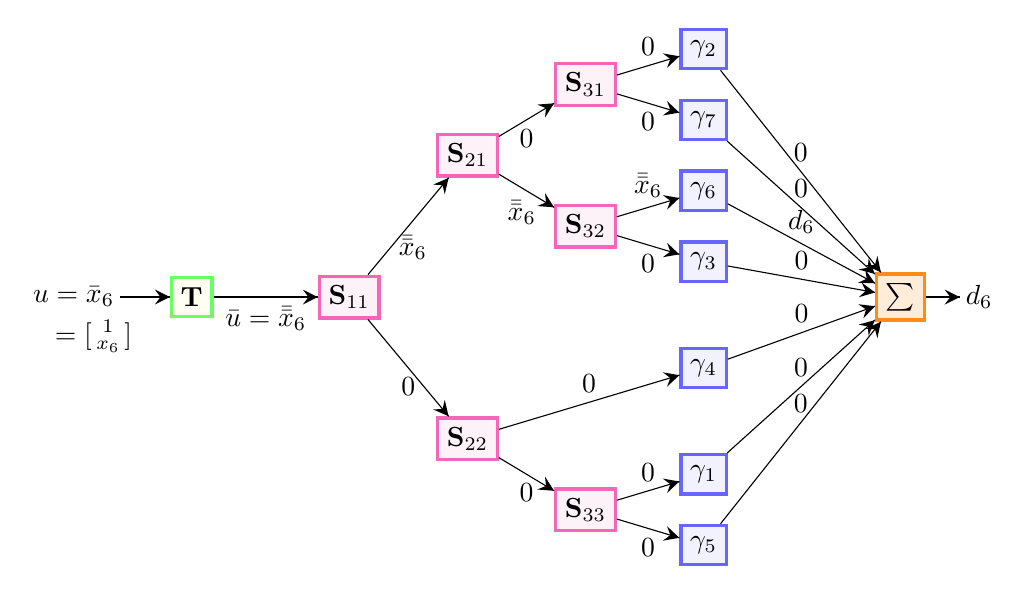
\begin{tikzpicture}[
				arrowstyle/.style={decoration={markings,mark=at position 1 with
						{\arrow[scale=1.7,>=stealth]{>}}},postaction={decorate}},
				roundnode/.style={circle, draw=blue!60, fill=blue!5, very thick, minimum size=2mm},
				squarednode/.style={rectangle, draw=green!60, fill=yellow!5, very thick, minimum size=5mm},
				squarednode2/.style={rectangle, draw=magenta!60, fill=magenta!5, very thick, minimum size=5mm},
				squarednode3/.style={rectangle, draw=blue!60, fill=blue!5, very thick, minimum size=5mm},
				squarednode4/.style={rectangle, draw=red!60, fill=red!5, very thick, minimum size=5mm},squarednode5/.style={rectangle, draw=orange!90, fill=orange!15, very thick, minimum size=5mm},]
				
				\node[inner sep=0pt, minimum size=3mm](n1x) at (-0.75,-0.5){$=[\begin{smallmatrix} 1 \\ x_6 \end{smallmatrix}]$};
				
				\node[inner sep=2pt, minimum size=3mm](n1) at (-1,0) {$u=\bar{x}_6$};
				\node[squarednode](t) at (0.5,0) {$\mathbf{T}$};
				\draw [arrowstyle](n1)--(t);
				\node[squarednode2](s11) at (2.5,0) {$\mathbf{S}_{11}$};
				\draw [arrowstyle](t)--node [below] {$\bar{u}=\bar{\bar{x}}_6$}(s11);
				\node[squarednode2](s21) at (4,1.8) {$\mathbf{S}_{21}$};
				\node[squarednode2](s22) at (4,-1.8) {$\mathbf{S}_{22}$};
				\draw [arrowstyle](s11)--node [below] {$\,\,\bar{\bar{x}}_6$}(s21);
				\draw [arrowstyle](s11)--node [below] {$0$}(s22);
				\node[squarednode2](s32) at (5.5,0.9) {$\mathbf{S}_{32}$};
				\node[squarednode2](s31) at (5.5,2.7) {$\mathbf{S}_{31}$};
				\node[squarednode2](s33) at (5.5,-2.7) {$\mathbf{S}_{33}$};
				
				\draw [arrowstyle](s21)--node [below] {$0$}(s31);
				\draw [arrowstyle](s21)--node [below] {$\!\!\bar{\bar{x}}_6$}(s32);
				\draw [arrowstyle](s22)--node [below] {$0$}(s33);
				
				\node[squarednode3](g2) at (7,3.15) {$\gamma_2$};
				\node[squarednode3](g7) at (7,2.25) {$\gamma_7$};
				\node[squarednode3](g6) at (7,1.35) {$\gamma_6$};
				\node[squarednode3](g3) at (7,0.45) {$\gamma_3$};
				\node[squarednode3](g5) at (7,-3.15) {$\gamma_5$};
				\node[squarednode3](g1) at (7,-2.25) {$\gamma_1$};
				\node[squarednode3](g4) at (7,-0.9) {$\gamma_4$};
				
				\draw [arrowstyle](s31)--node [above] {$0$}(g2);
				\draw [arrowstyle](s31)--node [below] {$0$}(g7);
				\draw [arrowstyle](s32)--node [above] {$\bar{\bar{x}}_6$}(g6);
				\draw [arrowstyle](s32)--node [below] {$0$}(g3);
				\draw [arrowstyle](s22)--node [above] {$0$}(g4);
				\draw [arrowstyle](s33)--node [above] {$0$}(g1);
				\draw [arrowstyle](s33)--node [below] {$0$}(g5);
				
%				\node[squarednode5](s32sum) at (8.5,0.9) {$\sum$};
%				\node[squarednode5](s31sum) at (8.5,2.7) {$\sum$};
%				\node[squarednode5](s33sum) at (8.5,-2.7) {$\sum$};
%				\node[squarednode5](s21sum) at (9.5,1.8) {$\sum$};
%				\node[squarednode5](s22sum) at (9.5,-1.8) {$\sum$};
				\node[squarednode5](finalsum) at (9.5,0) {$\sum$};
				\node[inner sep=2pt, minimum size=4mm](output) at (10.5,0) {$d_6$};
				\draw [arrowstyle](finalsum)--(output); 
				
				\draw [arrowstyle](g2)--node [above] {$0$}(finalsum);
				\draw [arrowstyle](g7)--node [above] {$0$}(finalsum);
				\draw [arrowstyle](g6)--node [above] {$d_6$}(finalsum);
				\draw [arrowstyle](g3)--node [above] {$0$}(finalsum);
				\draw [arrowstyle](g4)--node [above] {$0$}(finalsum);
				\draw [arrowstyle](g1)--node [above] {$0$}(finalsum);
				\draw [arrowstyle](g5)--node [above] {$0$}(finalsum);
				
%				\draw [arrowstyle](s33sum)--node [below] {$0$}(s22sum);
%				\draw [arrowstyle](s32sum)--node [below] {$d_6$}(s21sum);
%				\draw [arrowstyle](s31sum)--node [below] {$0$}(s21sum);
%				\draw [arrowstyle](s21sum)--node [below] {$d_6$}(finalsum);
%				\draw [arrowstyle](s22sum)--node [below] {$0$}(finalsum);
%				
				
	\end{tikzpicture}}}
	\caption{An example network architecture for the achievability result. The block $\mathbf{T}$ represents the transformation in Step 1. Blocks $\mathbf{S}_{ij}$ are the routing switches. Blocks $\gamma_i$ represent ReLU neurons with weights $\gamma_i$, and the $\sum$ block represents a ReLU neuron with all-one weights.}
	\label{fig:nnforachievability}
\end{figure}

In contrast to the deep and narrow architecture that is optimal for unconditional computation, the network that achieves the performance in Theorem \ref{th:reluach} is considerably wider but much shallower. In fact, the proof in Appendix \ref{sec:reluachthproofer} reveals that our network has width $O(n)$, with $O(n)$ nodes, and depth $O(\log n)$. These numbers are a consequence of the classical binary decision tree that we utilize in our network construction. Thanks to conditional computation, although the network has $O(n)$ nodes, every dataset pattern activates only $O(\log n)$ neurons instead of $O(\sqrt{n})$ neurons without conditional computation. Note that the function $\log n$ grows much slower than $\sqrt{n}$ so that the number of neurons activated by the conditional computation is asymptotically negligible relative to an unconditional network. Moreover, every neuron in the conditional computation network has a bounded number of $q$ weights. The two facts translate to  big savings in terms of the cost of computation, thanks to Theorem \ref{th:synth}. An interesting open problem that we shall leave as future work is whether one can achieve the same performance with a much smaller network size, e.g. with $O(\sqrt{n})$ neurons, which is known to be optimal. This will also help reduce the size of the network synthesized by Theorem \ref{th:synth}.



It should be mentioned that the bounds (\ref{eq:th1actneuronbound}) and (\ref{eq:th1actweightbound}) on the number of active neurons and weights as stated in Theorem \ref{th:reluach} holds only for input patterns that belong to the dataset. For such patterns, only one path from the input to the output of the neural network is activated. The global behavior of the neural network for arbitrary inputs is more complex. A careful analysis of the construction in Appendix \ref{sec:reluachthproofer}  reveals that near the decision boundaries (the lines in Fig. \ref{fig:divideandconquerb}), multiple paths of the network are activated, This will result in more active neurons and weights than what is suggested by the upper bounds in (\ref{eq:th1actneuronbound}) and (\ref{eq:th1actweightbound}), respectively. However, the measure of such pathological inputs can be made arbitrarily small by tuning the switches appropriately.

\label{sec:reluachthdiscuss}

\section{Ultimate Computational Limits to Memory Recall}
\label{sec:reluconv}
%\subsection{Main Result}
In the previous section, we showed that $O(\log n)$ operations is sufficient to perfectly recall one of $n$ input-output relationships. We now analyze the necessary number of operations per input for successful recall. Our main result in this context is provided by the following theorem.

\begin{theorem} 
\label{th:reluconv}
Let the input vectors $x_1,\ldots,x_n\in\mathbb{R}^p$ and the corresponding desired output vectors $d_1,\ldots,d_n\in\mathbb{R}$ satisfy the following  property:
\begin{itemize}
%\item For every $i\in\{1,\ldots,n\}$, every component of $x_i$ is non-zero.
\item The matrix $\Bigl[\begin{matrix}x_{i_1} & \cdots & x_{i_{p+1}} \\ d_{i_1} & \cdots & d_{i_{p+1}} \end{matrix} \Bigr]$ has rank $p+1$ for any subset $\{i_1,\ldots,i_{p+1}\}$ of $\{1,\ldots,n\}$. 
\end{itemize}
Suppose that a conditional network $f$ satisfies the desired input-output relationships: For every $i$, the output of the network is $d_i$ whenever the input is $x_i$. Also, assume that the number of operations performed on each $x_i$ is bounded above by some $\alpha \geq 0$. Then, we have $\alpha \geq \log_2 \frac{n}{p} \in O(\log n)$.
%Then, for any conditional network $f$ with $A(x_i;f) \leq \alpha,\,f(x_i) = d_i,\,\forall i$, we have $\alpha \geq \log_2 \frac{n}{p}$. 
\end{theorem}
\begin{proof}
%	Suppose, contrary to the statement of the theorem, that there are $\alpha < \log_2 \frac{n}{p}$ operations for each input. This means that there are less than $\alpha < \log_2 \frac{n}{p}$ comparisons for each input (including the comparisons that have to be made to implement the neuron activation functions). 	
	Since there are at most $\alpha$ operations per input, there are at most $\alpha$ comparisons per input as well, counting the comparisons needed to implement the neuron activation functions.  We can represent the entire conditional computation graph/network as a binary tree where the distance between the root and a leaf node is at most $\alpha$. This results in tree of at most $2^{\alpha}$ leaf nodes. Each node of the tree compares real numbers to intermediate variables, which are linear functions of network inputs or other intermediate variables. Assume now the contrary to the statement of the theorem, i.e. the number of operations for every input is at most $\alpha$, all input-output relationships are satisfied, but $n > 2^\alpha p$. Since there are at most $2^\alpha$ leaf nodes, there is at least one leaf node that admits $1+p$ inputs (i.e. there are $1+p$ input patterns of the dataset such that the corresponding path over the  tree ends at the leaf node). Without loss of generality, suppose the indices for these inputs are $\{1,\ldots,1+p\}$. Writing down the input output relationship of the network for the leaf node, we obtain
	\begin{align}
		\label{rouchecond}
		[d_1 \cdots d_{1+p}] = W_0[x_1 \cdots x_{1+p}]
	\end{align}
	for some $q\times p$ matrix $W_0$. This relationship follows, as by fixing 
	a path on the tree, we obtain the unique linear transformation $W_0$ that maps the inputs to the neural network to its outputs. According to the Rouch\'{e}–Capelli theorem \cite[Theorem 2.38]{shafarevich2012linear}, a necessary condition for the existence of $W_0$ to solve (\ref{rouchecond}) is 
	\begin{align}
		\mathrm{rank}([x_1 \cdots x_{p+1}]) = \mathrm{rank}\Bigl(\Bigl[\begin{matrix}x_1 & \cdots & x_{p+1} \\ d_{1} & \cdots & d_{p+1} \end{matrix} \Bigr]\Bigr).
	\end{align}
	On the other hand, as a result of the rank condition stated in the theorem, the left hand side rank evaluates to $p$, while the right hand side evaluates to $1+p$. We arrive at a contradiction, which concludes the proof of the theorem.
\end{proof}

%
%$x_1,\ldots,x_d$: input variables:
%
%$y_1,\ldots,y_m$: intermediate variables. these can only be linear functions of other $y_i$s and $x_i$s.
%
%Suppose we do at most $m$ operations for every input. Then, there are at most $m$ conditionings. for every input. 

%The proof relies on constructing a tree that provides a blueprint for the operation of a given neural network for a given dataset. By construction, the number of leaves of the tree equals the number of memory patterns that the neural network can store up to constant multipliers. Moreover, the number of leaves is bounded above by $2^{\alpha}$. Combining the two statements proves the theorem. The details are provided in Section \ref{sec:proofofthreluconv}.

The  condition on the dataset and the desired outputs that appear in the statement of Theorem \ref{th:reluconv} is, up to a certain extent, necessary for the lower bound to hold. For example, if the desired outputs can simply be obtained as a linear transformation of inputs, then one only needs to perform a constant number of operations for each input to obtain the desired outputs, and the lower bound becomes invalid. In this context, the rank condition ensures that subsets of outputs cannot be obtained as linear functions of inputs. However, it should also be mentioned that the condition is not particularly restrictive in limiting the class of datasets where the theorem holds. For example, if the components of the dataset members and the corresponding desired outputs are sampled in an independent and identically distributed manner over any continuous distribution with positive support, it can be shown that the rank condition will hold with probability $1$. Hence, it can be argued that almost all datasets satisfy the rank condition and thus obey the converse result.  

Corollary \ref{toyotacorolla} has shown that $n$ patterns can be memorized using  $O(\log n)$ operations per input. The matching $\Omega(\log n)$ lower bound in Theorem \ref{th:reluconv} proves that the $\Theta(\log n)$ rate is the best possible. However, the two results do not resolve how the number of operations should scale with respect to the input and output dimensions.\footnote{Although Theorem \ref{th:reluconv} only considers scalar desired outputs, it can easily be extended to the multi-dimensional case. In fact, a successful memorization of, say, two-dimensional output vectors with $o(\log n)$ active neurons would imply the successful memorization of scalar outputs with the same number of neurons (simply by ignoring the neurons that provide the second component of the output), contradicting Theorem \ref{th:reluconv}.} This aspect of the problem is left as future work.



%\begin{table}[t]
    \centering
    \footnotesize
    \begin{tabular}{c|cccc} \toprule
        Threshold & sFID & FS    & COUT & CD  \\ \midrule
        None      & 9.09 & 0.765 &0.532 & \textbf{2.66} \\
        0.05      & 6.83 & 0.787 &0.547 & 3.12 \\
        0.10      & 5.23 & 0.792 &0.565 & 2.75 \\
        0.15      & \textbf{4.62} & \textbf{0.797} &\textbf{0.564} & 2.82 \\ \midrule
        DiME      & 5.89 & 0.671 &0.444 & 3.27 \\ \bottomrule
    \end{tabular}
    \vspace{-0.1cm}
    \caption{Threshold ablation on CelebA (Age) with $l_2$ distance loss.}
    \label{tab-sup:t2}
\end{table}
\section{Conclusions}
We consider the phase-extraction problem, and we showed that, given a unitary $U = e^{i\pi H}$ and its inverse $U^{\dag}$, we could implement a block-encoding of $\phi(H)$ for some smooth function $\phi(x)$. The word `smooth' here means existence and continuity of the derivatives: the higher the number of continuous derivatives that a function has, the faster its Fourier sum (and thus the Laurent polynomial on the eigenphases) uniformly converges to that function. We are confident this can have many more applications beyond what is shown in this work. It is also worth remarking that Jackson showed that the convergence rate of a Fourier series is almost-optimal, in the sense that no trigonometric (or, equivalently, complex exponential) series can approximate the desired function faster, up to that $\log d$ factor~\cite[p.\ 21]{jacksonTheoryApproximation1930a}. Also remember that `smoothing' a function, i.e., replacing its derivative with a continuous function, does not give faster convergence for free in general, as its derivative will become steep in the points where we smooth out discontinuities, and this translates to a high Lipschitz constant: a~clear example is given by Eq.~\ref{eq:lipschitz-constant-recurrence-solution}, but in that case, fortunately, nothing depends on the size of the input $N$, and thus does not influence the asymptotic query complexity of Algorithm~\ref{alg:prop-sampling-qsp}, although the constant factor can become large even for $p = 20$. From a theoretical point of view, this work shows that, for any $\eta > 0$, there is an algorithm with query complexity 
$$\Tilde{\bigO}\left(\frac{1}{\bar{c}^{\frac{1}{2} + \eta}} \frac{1}{\epsilon^\eta} \right)$$
solving the proportional-sampling problem. This statement seems to suggest there exists an algorithm which directly solves the problem with $\eta = 0$, and an open question would be to find such algorithm.


It is also interesting to remark that Theorems~\ref{thm:haah-construction},~\ref{thm:haah-completion} indeed allow the construction for any $\phi$, even complex-valued, provided that its absolute value is reciprocal.

One could think that, in Section~\ref{sec:prop-sampling}, instead of using the linear function in the phase-extraction subroutine, we could approximate the square root and then apply the transformation directly on $e^{i \pi c(x)}$. However, in the case of proportional sampling this would be inconvenient, as the derivative of the square root function has a discontinuity with an infinite jump around 0, and we could not choose a constant $\delta$ if we had values of the oracle that are too close to $0$.

\newsavebox{\shortpagebox}


\subsubsection*{Acknowledgments}
This work was supported in part by National Science Foundation (NSF) under Grant CNS-2148182 and in part by Army Research Lab (ARL) under Grant W911NF-2120272.

\bibliographystyle{IEEEtran}
\bibliography{references}


% %\newpage
\section{Alternative Definitions}\label{sec:other-definitions-short}
In this section, we discuss other potential definitions of Leximin approximation that might be considered intuitive.
\eden{removed ack. for anonymous submission}
% \footnote{We thank Sylvain Bouveret for suggesting definitions \ref{altDef:5} and \ref{altDef:6}.}.
For each alternative, we provide an example that illustrates why we believe it is inappropriate and a conclusion based on that example.
It should be noted that in order to avoid confusion, the error parameter $\gamma \in (0,1)$ is used in the alternative definitions (instead of $\beta$), to emphasize that these are only alternatives we do not use.


\begin{potentialDefinition}\label{altDef:2}
    A solution $x$ is a $(1-\gamma)$-approximately optimal if given a Leximin-optimal solution, $x^*$, there exists an integer $k \in [n]$ such that: 
    \begin{align*}
    \forall j < k: & \valBy{j}{x} \geq (1-\gamma) \cdot \valBy{j}{x^*}\\
    & \valBy{k}{x} > \valBy{k}{x^*}
    \end{align*}
\end{potentialDefinition}

\paragraph{Bad example def. \ref{altDef:2}:} Consider the following example with three objectives:
\begin{align*}
    \max \quad &\{f_i(x) = x_i \mid \forall 1 \leq i \leq 3 \} \\ \tag{E1}\label{eq:alt-def-eaxmple-1}
    s.t. \quad  & 99 x_1 + x_2 \leq 100\\
    &  x_3 \leq 100\\
    & x \in \mathbb{R}^3_{+}
\end{align*}
The Leximin optimal solution $x^*$ is $(1,1, 100)$ and therefore, by taking $k$ to be $2$, we get that any solution that its minimum objective value is at least $(1-\gamma)$ and its second-smallest objective value is more than $1$ is considered $(1-\gamma)$-approximately optimal Leximin solution.
For instance, consider $\gamma = 0.1$, the solution $(0.9, 1.1, 1.1)$ should be considered a $0.9$-approximately optimal according to this definition.
However, it is easy to see that this solution is quite bad for $f_2$ who can achieve $10.9$ (higher by a factor $> 9$) and very bad for $f_3$ who can achieve $100$ (higher by a factor $>90$).
And so, it seem reasonable to require that a good definition will consider as many objectives as possible.
% \erel{What objective values exactly? Do you mean: as many objectives as possible?}
% \eden{yes. To myself: this comment might be relevant to other places..}

\paragraph{Conclusion def. \ref{altDef:2}:} An appropriate definition should take into account as many objectives as possible.

\begin{potentialDefinition}\label{altDef:1}
    A solution $x$ is a $(1-\gamma)$-approximately optimal if for a Leximin-optimal solution, $x^*$, and for each $j = 1, \dots, n$ the following holds: 
    \begin{align*}
        \valBy{j}{x} \geq (1-\gamma) \cdot \valBy{j}{x^*} 
    \end{align*}
\end{potentialDefinition}

\paragraph{Bad example def. \ref{altDef:1}:} 
% An error in the first objective value might cause the other values to increase significantly.
Consider example \eqref{eq:alt-def-eaxmple-1} again.
Here, as the optimal solution is $(1,1, 100)$, any solution that yields at least $(1-\gamma,1-\gamma, (1-\gamma)\cdot 100)$.
However, considering $\gamma = 0.1$, $f_2$ can again achieve $9.1$ which is higher by a factor $> 100$ than the value it got $0.1$.

\paragraph{Conclusion def. \ref{altDef:1}:} An appropriate definition should consider the fact that an error in one objective might change the optimal value of other objectives.
As a consequence, another conclusion is that an appropriate definition should not consider the optimal solution at all.



\begin{potentialDefinition}\label{altDef:3}
    A solution $x$ is a $(1-\gamma)$-approximately optimal 
    if it satisfies the following requirements:
    \begin{enumerate}
        \item The objective-function with the smallest objective value achieves at least its maximum value times $(1-\gamma)$:
        \begin{align*}
            \valBy{1}{x} \geq (1-\gamma) \cdot \valBy{1}{x^*} 
        \end{align*}
        
        \item Given all the solutions that satisfies the first condition, let $m_2$ be the highest second-smallest objective value.
        The objective-function with the second-smallest objective value achieves at least the $m_2$ times $(1-\gamma)$.
        
        \item Given all the solutions that satisfies the former conditions, let $m_3$ be the highest third-smallest objective value.
        The objective-function with the third-smallest objective value achieves at least the $m_3$ times $(1-\gamma)$.
        
        \item and so on.
    \end{enumerate}
\end{potentialDefinition}

\paragraph{Bad example def. \ref{altDef:3}:}
Consider the following example with only two objectives:
\begin{align*}
    \max \quad &\{f_1(x) = x_1, f_2(x)=x_2\} \\
    s.t. \quad  & 99 x_1 + x_2 \leq 100\\
    & x \in \mathbb{R}^2_{+}
\end{align*}
The Leximin-optimal solution is $(1,1)$. Consider $\gamma = 0.1$, according to part (1) of this definition, all solutions in which the smallest objective value is at least $(1-\gamma)=0.9$ should be considered in order to determine $m_2$.
So, in this case, $m_2$ is determined to be $100 - 0.9 \cdot 99 = 10.9$.
Then, according to part (2), in order to be considered a $0.9$-approximately optimal, the second value must be at least $0.9 \cdot 10.9 = 9.81$.
But, even the exact Leximin optimal solution does not satisfy this requirement, so this cannot be considered an approximation to Leximin optimal.

In general, this definition has the disadvantage of favoring solutions that give the lowest bounds to the objective functions considered in the earlier steps,  since this may enable to increase the values of the higher objectives.
According to the Leximin nature, the most important thing is to make the worst-off player as happy as possible (and then the second worst-off and so on), therefore, we emphasize the importance of this characteristic also in the definition of the approximated version.

\paragraph{Conclusion def. \ref{altDef:3}:} An appropriate definition should also capture the Leximin optimal solutions, and maintain the Leximin nature whenever possible.

% \eden{I think this definition is actually equivalent to our current... need to think about it again}
% \begin{potentialDefinition}\label{altDef:4}
%     A solution $x$ is a $\gamma$-approximately-optimal Leximin solution if it can be viewed as the result of this process:
%     \begin{enumerate}
%         \item Choose a solution in which the objective-function with the smallest objective value achieves at least the maximum value minus $\gamma$:
%         \begin{align*}
%             \valBy{1}{x} \geq \valBy{1}{x^*} - \gamma
%         \end{align*}
%         Let $z_1$ be the value it achieves (i.e., $\valBy{1}{x})$.
        
%         \item Consider all the solutions in which the objective-function with the smallest objective value achieves at least $z_1$ and let $m_2$ be the highest second-smallest objective value.
%         Then, choose a solution in which the objective-function with the second-smallest objective value achieves at least the $m_2$ minus $\gamma$.
%         Let $z_2$ be the value it achieves.
%         \item Consider all the solutions in which the objective-function, the smallest objective value achieves at least $z_1$ and the second-smallest objective value achieves at least $z_2$, and let $m_3$ be the highest third-smallest objective value.
%         Then, choose a solution in which the objective-function with the third-smallest objective value achieves at least the $m_3$ minus $\gamma$.
        
%         \item and so on...
%     \end{enumerate}
% \end{potentialDefinition}

% \paragraph{Bad example def. \ref{altDef:3}:} Although in this definition, the Leximin optimal solution is also approximately-optimal as we wanted, another issue arises.

% \begin{itemize}
%     \item \textbf{Bad example:} two solutions that meet this definition, but one of them is strictly better (by more than $\gamma$) than the other from some point.
%     \item \textbf{Conclusion:} an appropriate (good?) definition should determine between two solutions if possible. 
% \end{itemize}

% -----------------------------------
% \subsection{others}
% (From the correspondence of Erel with Lemaitre and Bouveret)

%----------------------------------
% need to think about a corresponding def for mult...
\begin{potentialDefinition}\label{altDef:5}
    A solution $x$ is a $(1-\gamma)$-approximately optimal if for a Leximin-optimal solution, $x^*$, and for each $j = 1, \dots, n$: 
    % in the addive version was $$$
    \begin{align*}
        % |\valBy{j}{x} - \valBy{j}{x^*}| \leq \gamma\\
         \max\{\valBy{j}{y},\valBy{j}{x}\}  \leq \frac{1}{1-\gamma} \cdot \min\{\valBy{j}{y},\valBy{j}{x}\}
    \end{align*}
\end{potentialDefinition}

\paragraph{Bad example and conclusion def. \ref{altDef:5}:}
This definition is close to definition \ref{altDef:1} but weaker, still the same example and conclusion apply.

\begin{potentialDefinition}\label{altDef:6}
    A solution $x$ is a $(1-\gamma)$-approximately optimal if given a Leximin-optimal solution, $x^*$, there exists an integer $k \in [n]$ such that: 
    \begin{align*}
    \forall j < k: & \valBy{j}{x} = \valBy{j}{x^*}\\
    & \valBy{k}{x} > (1-\gamma) \cdot \valBy{k}{x^*}
    \end{align*}
\end{potentialDefinition}
% \eden{I'm not sure it is well defined, since by decreasing $\gamma$ (for example) the second value might become smaller than the first.}

\paragraph{Bad example def. \ref{altDef:6}:} As in the case of definition \ref{altDef:2}, by taking a small $k$, we cannot distinguish between two solutions that satisfy this definition, but one of them should be definitely preferred.
Consider again the following example with three objectives, where:
\begin{align*}
    \max \quad &\{f_i(x) = x_i \mid \forall 1 \leq i \leq 3 \} \\
    s.t. \quad  & 9 x_1 + x_2 \leq 10\\
    &  x_3 \leq 100\\
    & x \in \mathbb{R}^3_{+}
\end{align*}
The Leximin optimal solution $x^*$ is $(1,1, 100)$ and therefore, by taking $k$ to be $2$, we get that any solution that its minimum value is $1$ and its second-smallest objective value is more than $(1-\gamma)$ is considered $(1-\gamma)$-approximately optimal.
As an example, the solution $(1, 1, 1)$ is considered $(1-\gamma)$-approximately-optimal Leximin solution (as $(1-\gamma) < 1$).
But it is easy to see that this solution is quite bad for $f_3$ (who can achieve $100$).

\paragraph{Conclusion def. \ref{altDef:6}:} Same as for def. \ref{altDef:2}, an appropriate definition should take into account as many objectives as possible.

% \begin{potentialDefinition}
%     OWA.
% \end{potentialDefinition}

%--------------------------

\begin{potentialDefinition}\label{altDef:7}
    A solution $x$ is a $(1-\gamma)$-approximately optimal if there is no other solution $y$ that is $(1-\gamma)$-Leximin preferred over it, where this relation is defined as follows: $y$ is preferred over $x$ if  there exists an integer $k \in [n]$ such that:
    \begin{align*}
        \forall j < k \colon \quad &   \max\{\valBy{j}{y},\valBy{j}{x}\}  \leq \frac{1}{(1-\gamma)} \cdot \min\{\valBy{j}{y},\valBy{j}{x}\}\\
        & \valBy{k}{y} > \frac{1}{(1-\gamma)} \cdot 
\valBy{k}{x}
    \end{align*}
     [This relation is related to a one suggested in \cite{kalai_lexicographic_2012}, it is described in more detail in the Related work Section]. 
\end{potentialDefinition}

\paragraph{Bad example and conclusion def. \ref{altDef:7}:} As with definition \ref{altDef:3}, here also, the Leximin optimal solution is not optimal according to this relation and it might favor solutions with lower smallest objective values. 
Consider again the following example:
\begin{align*}
    \max \quad &\{f_1(x) = x_1, f_2(x)=x_2\} \\
    s.t. \quad  & 99 x_1 + x_2 \leq 100\\
    & x \in \mathbb{R}^2_{+}
\end{align*}
Assume that $\gamma = 0.1$, the Leximin-optimal solution is $(1,1)$, but the solution $(0.9,10.9)$ is preferred over it according to this relation (since for $k=2$ we get that $\max\{0.9,1\} \leq \frac{1}{0.9}\cdot\min\{0.9,1\}$ and $10.9 > \frac{1}{0.9} \cdot 1$) and therefore, it is not approximately-optimal.



\section{The Approximate Leximin Order}\label{sec:approx-order-is-strict-partial}

Unlike the leximin order, $\leximinPreferred$, which is a strict \textbf{total} order, the approximate leximin order, $\alphaBetaPreferred$ for $\DEFmultApprox\in (0,1]$ and $\DEFadditiveApprox \geq 0$ is a strict \textbf{partial} order.
The difference is that in partial orders, not all vectors are comparable.
Consider for example the sorted vectors $(1,2)$ and $(1, 3)$. 
According to the leximin order, $(1,3)$ is clearly preferred (as $3>2$), but according to many approximate leximin orders neither one is preferred over the other, for example according to the orders $\alphaBetaPreferredParams{0.6}{0}$,$ \alphaBetaPreferredParams{1}{1}$ or $\alphaBetaPreferredParams{0.8}{0.5}$.
% (irreflexive, asymmetric and transitive).

An order is a strict partial order if it is irreflexive, transitive and asymmetric.
Lemma \ref{lemma:order-is-irreflexive} proves that the order is irreflexive, Lemma \ref{lemma:order-is-transitive} proves it is transitive, and Lemma \ref{lemma:order-is-asymmetric} proves that it is asymmetric.
% \erel{It would be good to show an example why this is not a total order.}

% need to prove irreflexive, asymmetric (we have already proved that it is transitive).

% ***[I thought it would be better to prove it on vectors (rather than "solutions") to make it as general as possible]\\

Let $\DEFmultApprox\in (0,1]$ and $\DEFadditiveApprox \geq 0$. 

\begin{lemma}\label{lemma:order-is-irreflexive}
    The approximate leximin order $\alphaBetaPreferred$ is irreflexive.
\end{lemma}

\begin{proof}
    % \eden{I used $x$ only to remind the reader what irreflexive is, maybe it should simply be in the lemma description}
    Let $x$ be a solution. We will show that $x \nAlphaBetaPreferred x$.
    As the definition requires that one component be \emph{strictly greater} than the other, it is trivial.
\end{proof}

\begin{lemma}\label{lemma:order-is-transitive}
    The approximate leximin order $\alphaBetaPreferred$ is transitive.
\end{lemma}

\begin{proof}
    Let $x,y$ and $z$ be solutions such that $x \alphaBetaPreferred y$ and $y \alphaBetaPreferred z$.
    We will prove that $x \alphaBetaPreferred z$.

    
    Since $x \alphaBetaPreferred y$, there exists an integer $ k_1 \in [n]$ such that:
    \begin{align*}
        \forall j<k_1 \colon &  \valBy{j}{x} \geq \valBy{j}{y}\\
            & \valBy{k_1}{x} > \frac{1}{\DEFmultApprox} \left( \valBy{k_1}{y} + \DEFadditiveApprox \right)
    \end{align*}
    And since $y \alphaBetaPreferred z$, there exists an integer $k_2 \in [n]$ such that:
    \begin{align*}
        \forall j<k_2 \colon &  \valBy{j}{y} \geq \valBy{j}{z}\\
            & \valBy{k_2}{y} > \frac{1}{\DEFmultApprox} \left( \valBy{k_2}{z} + \DEFadditiveApprox \right) 
    \end{align*}

    As $\DEFmultApprox \in (0,1]$ and $\DEFadditiveApprox \geq 0$, it follows that:
    \begin{align}\label{eq:trans-k-s}
        \valBy{k_1}{x} > \valBy{k_1}{y}, \Hquad \valBy{k_2}{y} >  \valBy{k_2}{z}
    \end{align}

    % Accordingly, if $k_1=k_2$, then this integer, denoted by $k$, allows us to conclude that $x \alphaBetaPreferred z$. 
    % By the definitions of $k_1$ and $k_2$, for any $j<k_1=k_2$ the required holds as $\valBy{j}{x} \geq \valBy{j}{y} \geq \valBy{j}{z}$.
    % In addition, $\valBy{k_1}{x}> \valBy{k_1}{y}$ by equation \ref{eq:trans-k-s}
    % $ > \frac{1}{\DEFmultApprox} \left( \valBy{k_1}{y} + \DEFadditiveApprox \right)$ and nd  and 
    
    Let $k = \min\{k_1,k_2\}$.
    
    If $k = k_1$, by the definition of $k_1$, $\valBy{k}{x} > \frac{1}{\DEFmultApprox} \left( \valBy{k}{y} + \DEFadditiveApprox \right)$.
    However, $\valBy{k}{y} \geq \valBy{k}{z}$, by definition if $k<k_2$ and by equation \ref{eq:trans-k-s} if $k=k_2$. \ref{eq:transitive-k}
    Therefore, $\valBy{k}{x} > \frac{1}{\DEFmultApprox} \left( \valBy{k}{z} + \DEFadditiveApprox \right)$.
    
    Otherwise, if $k=k_2$, by the definition of $k_2$, $\valBy{k}{y} > \frac{1}{\DEFmultApprox} \left( \valBy{k}{z} + \DEFadditiveApprox \right)$. But, $\valBy{k}{x} \geq \valBy{k}{y}$, by definition if $k<k_1$ and by equation \ref{eq:trans-k-s} if $k=k_1$. Again, we can conclude that $\valBy{k}{x} > \frac{1}{\DEFmultApprox} \left( \valBy{k}{z} + \DEFadditiveApprox \right)$.

     In addition, for each $j<k$, since $j< k_1$ and $j < k_2$, by definition the following holds:
    \begin{align}\label{eq:transitive-k}
        \valBy{j}{x} \geq \valBy{j}{y} \geq \valBy{j}{z}
    \end{align}
    So, $k$ is an integer that satisfy all the requirements, and so, $x \alphaBetaPreferred z$.
    \end{proof}
    

    
    \begin{lemma}\label{lemma:order-is-asymmetric}
        The approximate leximin order $\alphaBetaPreferred$ is asymmetric.
    \end{lemma}
    
    \begin{proof}
        Let $x$ and $y$ be solutions such that $x \alphaBetaPreferred y$. We will show that $y \nAlphaBetaPreferred x$. 
        Assume by contradiction that $y \alphaBetaPreferred x$. 
        From Lemma \ref{lemma:order-is-transitive}, this relation is transitive. Therefore, since $x \alphaBetaPreferred y$ and $y \alphaBetaPreferred x$, also $x \alphaBetaPreferred x$.
        But, from Lemma \ref{lemma:order-is-irreflexive}, this relation is irreflexive --- a contradiction.
    \end{proof}
\section{Proof of Theorem \ref{th:main}}\label{sec:algo-sec-proofs}
\eden{should probably change the title}

This section is dedicated to proving Theorem \ref{th:main}.
To this end, we use another equivalent representation of \eqref{eq:sums-OP}, which was also introduced by \cite{Ogryczak_2006} 
(we provide the proof of equivalence in Appendix \ref{sec:equivalent-proofs}). 
\erel{Can't we just use it directly instead of P2?}
% (here also, the variables are $\ztVar{x}$ and $x$, and $z_1, \ldots z_{t-1}$ are constants)
\begin{align*}
    \max \quad &z_t \tag{P2-compact}\label{eq:compact-OP} \;\;
        s.t. &\quad  & (1) \quad x \in S\\
                    &&& (\Tilde{2}) \quad \sum_{i=1}^{\ell} \valBy{i}{x} \geq \sum_{i=1}^{\ell}  z_i && \ell = 1,\ldots, t-1 \nonumber\\
                    &&& (\Tilde{3}) \quad \sum_{i=1}^{t} \valBy{i}{x} \geq \sum_{i=1}^{t}  z_i
\end{align*}
In this problem, constraints $(\hat{2})$ and $(\hat{3})$ are replaced by  $(\Tilde{2})$ and $(\Tilde{3})$, respectively.  
The difference is that
$(\hat{2})$ gives, for each $\ell$, a lower bound on the sum for \emph{any} set of $\ell$ objective functions; whereas $(\Tilde{2})$ only considers the sum of the $\ell$ \emph{smallest} such values.  
% However, since the constraints set the same lower bound on this sum, the constraints are equivalent.  
Similarly for $(\hat{3})$ and $(\Tilde{3})$. 
Since  the problems are equivalent, a solver, either exact or approximate, for one can be used as a solver, with the same level of accuracy, for the other (Lemma \ref{lemma:solver-equivalent-prob}). 
Therefore, as \eqref{eq:compact-OP} is equivalent to \eqref{eq:sums-OP}, which, in turn, is equivalent to \eqref{eq:vsums-OP}, in proving the theorem we may assume that \textsf{OP} is an approximation procedure for \eqref{eq:compact-OP}.  
This will simplify the proofs. \eden{I added the line from the comment back, isn't it important to explain why we need this representation?}

% \erel{*** I do not understand. We say that P1 and P2 are equivalent with an exact solver, but not with an approximate solver. Here, we claim that P3 and P2-compact are equivalent, but this is true only with an exact solver. Don't we have to prove that they are equivalent also with an approximate solver? ***}

We denote $\retSol := x_n$ = the solution $x$ attained at the last iteration ($t=n$) of the algorithm. 

Following are some observations regarding the set of feasible solutions in each iteration, their objective values, and the solution $\retSol$ that will be useful later on.

% For any constants $z_1,\ldots, z_{t-1}$,
% any vector $x \in S$ that satisfies constraint $(\Tilde{2})$ of \eqref{eq:compact-OP} 
% is feasible to this problem.
% This is because any solution $x \in S$ can satisfy constraint $(\Tilde{3})$ with a small enough assignment to the variable $z_t$. \eden{I'm not sure how to explain it....}
\begin{observation}\label{obs:feasi-and-constraint2}
For any constants $z_1,\ldots, z_{t-1}$,
any vector $x \in S$ that satisfies constraint $(\Tilde{2})$ of \eqref{eq:compact-OP} 
can be a part of a feasible solution $(x,z_t)$ for any $z_t \leq \sum_{i=1}^{t} \valBy{i}{x} - \sum_{i=1}^{t-1} z_i$.
\end{observation}

Since $\retSol$ is a feasible solution of \eqref{eq:compact-OP} in iteration $n$, and as each
iteration only adds new constraints to $(\Tilde{2})$, it follows that $\retSol$ is also a feasible solution of \eqref{eq:compact-OP} in any iteration $1 \leq t\leq n$. 
\begin{observation}\label{obs:retSol-solves-any-t}
$\retSol$ is a feasible solution of \eqref{eq:compact-OP} in any iteration $1 \leq t\leq n$.
\end{observation}

Now, consider the problem \eqref{eq:compact-OP} that was solved in iteration $t$.
Here, $z_t$ is a \emph{variable} and $z_1, \ldots z_{t-1}$ are constants.
The objective of this problem is $\max z_t$, and the only constraint that includes the variable $z_t$ is  $(\Tilde{3})$.
Therefore, rearranging it to $\sum_{i=1}^{t} \valBy{i}{x} - \sum_{i=1}^{t-1}  z_i\geq z_t$, allows us to conclude that the objective value is determined by the left side of this inequality (as $z_t$ is maximized when the inequality turns to equality).
\begin{observation}\label{obs:obj-value}
The objective value obtained by a feasible solution $x$ to the problem \eqref{eq:compact-OP} that was solved in iteration $t$ is $\sum_{i=1}^{t} \valBy{i}{x} - \sum_{i=1}^{t-1}  z_i$.
\end{observation}

Lastly, as the value obtained as a $(\multApprox, \additiveApprox)$-approximation for this problem is the \emph{constant} $z_t$, the optimal value is at most $\frac{1}{\multApprox} (z_t+\additiveError)$. 
Consequently, the objective value of any feasible solution is at most this value.
Since $\retSol$ is feasible for any iteration $t$ (Observation \ref{obs:retSol-solves-any-t}) and since its objective is $\sum_{i=1}^t \valBy{i}{\retSol} - \sum_{i=1}^{t-1} z_i$ (Observation \ref{obs:obj-value}), we can conclude:

\begin{observation}\label{obs:obj-xt-to-zt}
    The objective value obtained by $\retSol$ to the problem \eqref{eq:compact-OP} that was solved in iteration $t$ is at most $\frac{1}{\multApprox} (z_t+\additiveError)$. That is:
    \begin{align*}
        \sum_{i=1}^t \valBy{i}{\retSol} - \sum_{i=1}^{t-1} z_i \leq \frac{1}{\multApprox} \left(z_t+\additiveError \right).
    \end{align*}
\end{observation}

% This conclusion also implies that for any $1 \leq t \leq n$, the solution $(x_t, z_t)$ that that was outputted for \eqref{eq:compact-OP} in iteration $t$, satisfies constraint $(\Tilde{3})$ as equality. That is:
% \begin{observation}\label{obs:equality-xt-zt}
% For any $1 \leq t \leq n$,  $\sum_{i=1}^{t} \valBy{i}{x_t} = \sum_{i=1}^{t}  z_i$.
% \end{observation}



%%%
% OVERALL EXPLANATION 
We start with Lemmas \ref{lemma:beta-vk}-\ref{lemma:fk-to-all}, which establish a relationship between the $k$-th least objective value obtained by $\retSol$ 
% ($\valBy{k}{\retSol}$) 
and the difference between the sum of the $(k-1)$ least objective values obtained by $\retSol$ and the sum of the $(k-1)$ first $z_i$ values.
% ($\sum_{i=1}^{k-1}\valBy{k}{\retSol} - \sum_{i=1}^{k-1}z_i$). 
Theorem \ref{th:main} then uses this relation to prove that the existence of another solution that would be $\left(\frac{\multApprox^2}{1-\multApprox + \multApprox^2}, \frac{\multApprox(2-\multApprox)\additiveApprox}{1-\multApprox +\multApprox^2}\right)$-preferred over $\retSol$ would lead to a contradiction.

For clarity, throughout the proofs, we denote the multiplicative error factor by $\multError = 1-\multApprox$.

% LEMMAS.
% BLAH BLAH.

\begin{lemma}\label{lemma:beta-vk}
    For all $k\in[n]$, 
    \begin{align*}
        \multError \valBy{k}{\retSol} \geq \left(\sum_{i=1}^k \valBy{i}{\retSol} - \sum_{i=1}^k z_i\right) -\multError \left(\sum_{i=1}^{k-1} \valBy{i}{\retSol} - \sum_{i=1}^{k-1} z_i\right) -\additiveError
    \end{align*}
\end{lemma}

\begin{proof}
By Observation \ref{obs:obj-xt-to-zt},
    \begin{align*}
         &\sum_{i=1}^k \valBy{i}{\retSol} - \sum_{i=1}^{k-1} z_i \leq \frac{1}{\multApprox} \left(z_k + \additiveError \right) = \frac{1}{1-\multError} \left(z_k + \additiveError \right)\\
         &\Rightarrow z_k +\additiveError \geq (1-\multError) \left(\sum_{i=1}^{k} \valBy{i}{\retSol} - \sum_{i=1}^{k-1}  z_i\right)\\
        &\Rightarrow z_k +\additiveError\geq \left(\sum_{i=1}^{k} \valBy{i}{\retSol} - \sum_{i=1}^{k-1}  z_i\right) - \multError \left(\sum_{i=1}^{k} \valBy{i}{\retSol} - \sum_{i=1}^{k-1}  z_i\right)\\
        &\Rightarrow \multError \valBy{k}{\retSol} \geq \left(\sum_{i=1}^k \valBy{i}{\retSol} - \sum_{i=1}^k z_i\right) -\multError \left(\sum_{i=1}^{k-1} \valBy{i}{\retSol} - \sum_{i=1}^{k-1} z_i\right) -\additiveError.
        \qedhere
    \end{align*}
\end{proof}


\begin{lemma}\label{lemma:beta-sums-to-diff}
    For all $k\in[n]$, 
    \begin{align*}
        \sum_{i=1}^k \multError^{i} \valBy{k-i+1}{\retSol} \geq \sum_{i=1}^k \valBy{i}{\retSol} - \sum_{i=1}^{k} z_i -\additiveError
    \end{align*}
\end{lemma}

\begin{proof}
    The proof is by induction on $k$.
    For $k=1$ the claim follows directly from Lemma \ref{lemma:beta-vk}.
    Assuming the claim is true for $1,\ldots k-1$, we show it is true for $k$:
    \begin{align*}
        &\sum_{i=1}^k \multError^{i} \valBy{k-i+1}{\retSol} = \multError \valBy{k}{\retSol} + \sum_{i=2}^k \multError^{i} \valBy{k-i+1}{\retSol}\\
        &= \multError \valBy{k}{\retSol} + \sum_{i=1}^{k-1} \multError^{i+1} \valBy{k-(i+1)+1}{\retSol} \\
        &= \multError \valBy{k}{\retSol} + \multError \sum_{i=1}^{k-1} \multError^{i} \valBy{(k-1) -i+1}{\retSol}\\
        &= \multError \valBy{k}{\retSol} + \multError \left(\sum_{i=1}^{k-1} \valBy{i}{\retSol} - \sum_{i=1}^{k-1} z_i\right) && \text{(by induction assumption)}\\
        &\geq \left(\sum_{i=1}^k \valBy{i}{\retSol} - \sum_{i=1}^k z_i\right) -\multError \left(\sum_{i=1}^{k-1} \valBy{i}{\retSol} - \sum_{i=1}^{k-1} z_i\right)-\additiveError  \\
        & \quad +  \multError \left(\sum_{i=1}^{k-1} \valBy{i}{\retSol} - \sum_{i=1}^{k-1} z_i\right) && \text{(by Lemma \ref{lemma:beta-vk})} \\
        &= \sum_{i=1}^k \valBy{i}{\retSol} - \sum_{i=1}^{k} z_i -\additiveError.
        \qed
    \end{align*}
\end{proof}


\begin{lemma}\label{lemma:fk-to-all}
    For all $1<k \leq n$, 
    \begin{align*}
        \frac{\multError}{1-\multError} \valBy{k}{\retSol} \geq \sum_{i=1}^{k-1}\valBy{i}{\retSol} - \sum_{i=1}^{k-1}z_i - \additiveError
    \end{align*}
\end{lemma}

\begin{proof}
    First, notice that since $k \geq (k-1)-i+1$ for any $1\leq i \leq k$ and as the function $\valBy{i}$ represents the $i$-th smallest objective value, also:
    \begin{align}\label{eq:increase-by-obj-size}
        \forall 1\leq i \leq k \colon \quad \valBy{k}{\retSol} \geq \valBy{(k-1)-i+1}{\retSol}
    \end{align}
    In addition, consider the geometric series with a first element $1$, a ratio $\multError$, and a length $(k-1)$. 
    As $\multError < 1$, its sum can be bounded in the following way:
    \begin{align}\label{eq:geometric-series-beta}
        \sum_{i=1}^{k-1} \multError^{i-1} = \frac{1-\multError^{k-1}}{1-\multError} < \lim_{k \to \infty}\frac{1-\multError^{k-1}}{1-\multError} = \frac{1}{1-\multError}
    \end{align}
    
    Now, the claim can be concluded as follows:
    \begin{align*}
        & \frac{\multError}{1-\multError}\valBy{k}{\retSol} = \multError \left(\frac{1}{1-\multError} \valBy{k}{\retSol} \right)\\
        & > \multError \left(\sum_{i=1}^{k-1} \multError^{i-1} \valBy{k}{\retSol} \right) && \text{(by Equation \eqref{eq:geometric-series-beta})}\\
        & \geq  \multError \left(\sum_{i=1}^{k-1} \multError^{i-1} \valBy{(k-1)-i+1}{\retSol} \right) && \text{(by Equation \eqref{eq:increase-by-obj-size})}\\
        &= \sum_{i=1}^{k-1} \multError^{i} \valBy{(k-1)-i+1}{\retSol} \\
        &\geq \sum_{i=1}^{k-1}\valBy{i}{\retSol} - \sum_{i=1}^{k-1}z_i - \additiveError && \text{(by Lemma \ref{lemma:beta-sums-to-diff})}
\end{align*}
\erel{Formally, Lemma \ref{lemma:beta-sums-to-diff} is for $k\geq 1$, and we apply it for $k-1$, which might be $0$.}\eden{I tried to fixed it, is it better?}
\end{proof}



%------
% thm.

We are now ready to prove the Theorem \ref{th:main}.
\begin{proof}[Proof of Theorem \ref{th:main}]
% \eden{I'm not sure if we should write again about the claim with $\multApprox$}
Recall that the claim is that $\retSol$ is a $\left(\frac{\multApprox^2}{1-\multApprox + \multApprox^2}, \frac{\multApprox(2-\multApprox)\additiveApprox}{1-\multApprox +\multApprox^2}\right)$-approximation.

For brevity, we define the following constants:
\begin{align*}
    \Delta^{mult} = \frac{\multApprox}{1-\multApprox + \multApprox^2}, \quad  \Delta^{add} = \frac{\multApprox(2-\multApprox)}{1-\multApprox +\multApprox^2}
\end{align*}
Accordingly, we need to prove that $\retSol$ is a $\left(\Delta^{mult} \cdot \multApprox, \Delta^{add}\cdot\additiveApprox\right)$-approximation.

We prove the following equation, that will be helpful later:
\begin{align}\label{equ:mu}
\frac{1}{\Delta^{mult} \cdot \multApprox} = \frac{1-\multError +\multError^2}{(1-\multError)^2}
\end{align}
This is true because
\begin{align*}
    &\Delta^{mult} \cdot \multApprox =   \frac{\multApprox^2}{1-\multApprox + \multApprox^2} && \text{(Definition of $\Delta^{mult}$)} \\
    &= \frac{(1-\multError)^2}{\multError +(1-\multError)^2} = \frac{(1-\multError)^2}{1-\multError +\multError^2} &&\text{(since $\multApprox = 1-\multError$)}\\
    & \Rightarrow \frac{1}{\Delta^{mult} \cdot \multApprox} = \frac{1-\multError +\multError^2}{(1-\multError)^2}
    \end{align*}
    Another equation that will be useful later is:
    \begin{align}\label{eq:additive-error}
        \frac{\Delta^{add}}{\Delta^{mult}\cdot \multApprox}  = \frac{1+\multError}{1-\multError}.
    \end{align}
    The reason for this is that
    \begin{align*}
        &\frac{\Delta^{add}}{\Delta^{mult}\cdot \multApprox} =\frac{1-\multApprox + \multApprox^2}{\multApprox^2} \cdot \frac{\multApprox(2-\multApprox)}{1-\multApprox +\multApprox^2}&& \text{(Definitions of $\Delta^{mult}$ and $\Delta^{add}$)}\\
        &=\frac{\multApprox(2-\multApprox)}{\multApprox^2} = \frac{(1-\multError)(1 + \multError)}{(1-\multError)^2} =\frac{1+\multError}{1-\multError}  &&\text{(since $\multApprox = 1-\multError$)}
    \end{align*}

    Now, suppose by contradiction that $\retSol$ is \emph{not} $\left(\Delta^{mult} \cdot \multApprox, \Delta^{add}\cdot\additiveApprox\right)$-approximately-optimal.
    By definition, this means there exists a solution $y \in S$  that is $\left(\Delta^{mult} \cdot \multApprox, \Delta^{add}\cdot\additiveApprox\right)$-preferred over it.
    That is, there exists an integer $1 \leq k \leq n$ such that:
    \begin{align*}
        \forall j < k \colon &\valBy{j}{y} \geq \valBy{j}{\retSol};\\
        & \valBy{k}{y} > \frac{1}{\Delta^{mult} \cdot\multApprox} \left(\valBy{k}{\retSol} + \Delta^{add} \cdot\additiveError \right).
    \end{align*}

    Since $\retSol$ was obtained in \eqref{eq:compact-OP} that was solved in the last iteration $n$, it is clear that $\sum_{i=1}^k \valBy{i}{\retSol} \geq \sum_{i=1}^{k} z_i$ (by constraint $(\Tilde{2})$ if $k<n$ and $(\Tilde{3})$ otherwise).
    Which implies:
    \begin{align}\label{eq:fk-to-zk}
        \sum_{i=1}^k \valBy{i}{\retSol} - \sum_{i=1}^{k-1} z_i \geq z_k
    \end{align}

    Now, consider \eqref{eq:compact-OP} that was solved in iteration $k$.
    By Observation \ref{obs:retSol-solves-any-t}, $\retSol$ is feasible to this problem.
    As the $(k-1)$ smallest objective values of $y$ are at least as high as those of $\retSol$, it is easy to conclude that $y$ also satisfies constraints $(\Tilde{2})$ of this problem; since, for any $\ell < k$:
    \begin{align*}
        \sum_{i=1}^{\ell} \valBy{i}{y} \geq\sum_{i=1}^{\ell} \valBy{i}{\retSol} \geq \sum_{i=1}^{\ell} z_i
    \end{align*}
    Therefore, by Observation \ref{obs:feasi-and-constraint2}, $y$ is also feasible to this problem. 

    If $k=1$, the objective value $y$ in this problem is $\valBy{1}{y}$ (Observation \ref{obs:obj-value}).
    In addition, $\valBy{1}{\retSol} \geq z_1$ by equation \ref{eq:fk-to-zk}. As $\Delta^{mult}\geq 0$ and $\Delta^{add}\geq 0$, it follows that:
    \begin{align*}
        \valBy{1}{y}> \frac{1}{\Delta^{mult} \cdot\multApprox} \left(\valBy{1}{\retSol} + \Delta^{add} \cdot\additiveError \right)\geq \frac{1}{\multApprox} \left(z_1 + \additiveError \right)
    \end{align*}
    But, $z_1$ was obtained as an approximation for this problem, therefore the optimal value is at most $\frac{1}{\multApprox}\left(z_1 + \additiveError \right)$ --- a contradiction.

    
    Otherwise, $k>1$, we shall now see that in this case $y$ also satisfies the following:
    \begin{align}\label{eq:yk-to-sum}
        \valBy{k}{y} > \frac{1}{1-\multError} \valBy{k}{\retSol} + \frac{\multError}{1-\multError}\sum_{i=1}^{k-1}\valBy{i}{\retSol} - \frac{\multError}{1-\multError} \sum_{i=1}^{k-1}z_i  +\frac{1}{1-\multError}\cdot\additiveError
    \end{align}
    this is true because
    \begin{align*}
        &\valBy{k}{y} > \frac{1}{ \Delta^{mult} \cdot\multApprox} \left(\valBy{k}{\retSol} + \Delta^{add}\cdot \additiveError \right) && \text{(Definition of $y$ for $k$)}\\
        &= \frac{1-\multError +\multError^2}{(1-\multError)^2} \valBy{k}{\retSol}+ \frac{\Delta^{add}}{\Delta^{mult} \multApprox}\cdot\additiveError && \text{(by Equation \ref{equ:mu})}\\
        &= \frac{1-\multError +\multError^2}{(1-\multError)^2} \valBy{k}{\retSol}+ \frac{1+\multError}{1-\multError}\cdot\additiveError && \text{(by Equation \ref{eq:additive-error})} \erel{???}\\
        &\geq\frac{1}{1-\multError} \valBy{k}{\retSol} + \frac{\multError}{1-\multError}\left(\sum_{i=1}^{k-1}\valBy{i}{\retSol} - \sum_{i=1}^{k-1}z_i-\additiveError\right) +\frac{1+\multError}{1-\multError}\cdot\additiveError && \text{(by Lemma \ref{lemma:fk-to-all} for $k>1$)}\\
        & = \frac{1}{1-\multError} \valBy{k}{\retSol} +\frac{\multError}{1-\multError}\sum_{i=1}^{k-1}\valBy{i}{\retSol} - \frac{\multError}{1-\multError} \sum_{i=1}^{k-1}z_i +\frac{1}{1-\multError}\cdot\additiveError &&\erel{???}\text{\eden{is it more clear?}}
    \end{align*}    
    
    We compute the objective value of $y$, which is $\sum_{i=1}^k \valBy{i}{y} - \sum_{i=1}^{k-1} z_i$ (by Observation \ref{obs:obj-value}):  
    \begin{align*}
        &\sum_{i=1}^k \valBy{i}{y} - \sum_{i=1}^{k-1} z_i=\sum_{i=1}^{k-1} \valBy{i}{y} - \sum_{i=1}^{k-1} z_i + \valBy{k}{y}\\
        &\geq \sum_{i=1}^{k-1} \valBy{i}{\retSol} - \sum_{i=1}^{k-1} z_i + \valBy{k}{y} && \text{(Definition of $y$ for $j<k$)}\\
        &> \sum_{i=1}^{k-1} \valBy{i}{\retSol} - \sum_{i=1}^{k-1} z_i + \frac{1}{1-\multError} \valBy{k}{\retSol} \\
        & \quad + \frac{\multError}{1-\multError}\sum_{i=1}^{k-1}\valBy{i}{\retSol} - \frac{\multError}{1-\multError}\sum_{i=1}^{k-1}z_i +\frac{1}{1-\multError}\cdot\additiveError && \text{(by Equation \ref{eq:yk-to-sum})}\\
        & = \frac{1}{1-\multError} \left(\sum_{i=1}^k \valBy{k}{\retSol} - \sum_{i=1}^{k-1}z_i + \additiveError\right) &&\text{(since  $1+\frac{\multError}{1-\multError} = \frac{1}{1-\multError}$)}\erel{???}\text{\eden{is it more clear?}}
        \\
        &\geq \frac{1}{1-\multError} \left(z_k +\additiveError\right) && \text{(by Equation \ref{eq:fk-to-zk}) }
    \end{align*}
    \eden{I'm not sure why to comment the lines, shouldn't we explain why it is a contradiction?how is the following?}
    % \emark{However, the approximately-optimal solution obtained for this problem during the algorithm run is $z_k$, so the optimal value is at most $\frac{1}{(1-\multError)}\left(z_k+\additiveError\right)$.
    % But, as we shall see, the objective $y$ yields in this problem, $\sum_{i=1}^k \valBy{i}{y} - \sum_{i=1}^{k-1} z_i$ (by Observation \ref{obs:obj-value}), is higher than this value, which is of course a contradiction:}
    However, the approximately-optimal value obtained for this problem during the algorithm run is $z_k$, so the optimal value is at most $\frac{1}{(1-\multError)}\left(z_k+\additiveError\right)$, which is, again, a contradiction.
    
\end{proof}

\section{Proof of Theorem \ref{th:app-main}}\label{sec:app-sec-proofs}
% \eden{should probably change the title}

% Agents are assumed to care only about their own share (allowing us to use the following abuse of notation in which $u_j$ takes a bundle $b$ of items), their utilities are assumed to be normalized ($u_j(\emptyset) = 0$), monotone ($u_j(b_1) \leq u_j(b_2)$ if $b_1 \subseteq b_2$), and submodular ($u_j(b_1) + u_j(b_2) \geq u_j(b_1 \cup b_2) + u_j(b_1 \cap b_2)$ for any bundles $b_1,b_2$).
% It is assumed that each agent assigns a positive utility to the set of all items.
% The utilities $(u_i)_{i=1}^n$ are assumed to be given in the \emph{value oracle model}, meaning that we do not have a direct access to them, but only to an oracle that indicates the value of an agent from a given simple allocation.
% % \eden{z1 > 0}

This section proves Theorem \ref{th:app-main}:
suppose we are given a randomized algorithm that returns a simple allocation that approximates the utilitarian welfare with multiplicative error $\multError$ (with success probability $p$).
Then, Algorithm \ref{alg:basic-ordered-Outcomes} can be used to obtain a stochastic allocation that approximates leximin with a multiplicative error of at most $\frac{\multError}{1-\multError +\multError^2}$ (with the same probability).

% title: the specific problem as P3
As we saw in Section \ref{sec:algo-short}, an approximation to leximin can be obtained by providing a procedure \textsf{OP} to approximate \eqref{eq:vsums-OP}  (Theorem \ref{th:main}), which, under these particular settings, becomes:
% \erel{Why do you call it "configuration LP"? I think this term refers to something else: \url{https://en.wikipedia.org/wiki/Configuration_linear_program}}
\begin{align}
&\max \quad z_t \quad s.t. \tag{\progAppFirst}\label{eq:app-vsums-OP}\\
& (\text{\progAppFirst.1.1}) \Hquad \sum_{A \in \mathcal{A}} p_d(A) = 1 \nonumber\\
& (\text{\progAppFirst.1.2}) \Hquad p_d(A) \geq 0  && \forall A \in \mathcal{A} \nonumber\\
& (\text{\progAppFirst.2}) \Hquad \ell y_{\ell} - \sum_{j=1}^n m_{\ell,j}\geq \sum_{i=1}^{\ell}  z_i && \forXinY{\ell}{t-1} \nonumber \\
& (\text{\progAppFirst.3}) \Hquad t y_t - \sum_{j=1}^{n} m_{t,j} \geq \sum_{i=1}^{t}  z_i \nonumber \\
& (\text{\progAppFirst.4}) \Hquad m_{\ell,j} \geq y_{\ell} - \sum_{A \in \mathcal{A}}p_d(A) \cdot u_j(A)  && \forXinY{\ell}{t},\Hquad \forXinY{j}{n} \nonumber \\
& (\text{\progAppFirst.5}) \Hquad m_{\ell,j} \geq 0  && \forXinY{\ell}{t},\Hquad \forXinY{j}{n} \nonumber
\end{align}
Here the variables are $p_d(A)$ for any simple allocation $A \in \mathcal{A}$, $\ztVar{}$, and $y_{\ell}$ and $m_{\ell,j}$ for all $\ell \in [t]$ and $ j\in [n]$; and the values $z_1, \ldots z_{t-1}$ are constants.
Notice that it is a \emph{linear program} that has a polynomial number of constraints thanks to \eqref{eq:vsums-OP} representation, but an exponential number of variables (since there is a variable $p_d(A)$ for each simple allocation).
So, it is unclear how to approach it directly in polynomial time.
% \eden{here?}
In addition, it means that the output size is exponential in $n$.
To deal with this issue, the solutions are considered in \emph{sparse form} --- a list of the variables with positive values, along with their values.
Accordingly, if a solution has only a polynomial number of variables with positive values it can be represented by a polynomial size.
We will later see that the procedure described in this section returns such a solution in polynomial time.
% \eden{should write something about the output size, as \cite{kawase_max-min_2020}}

% title: baseline
% \erel{I would move the following paragraph upwards}
With $t=1$, \eqref{eq:app-vsums-OP} can be viewed as the problem of egalitarian welfare maximization, indeed, Kawase and Sumita \cite{kawase_max-min_2020} who studied this problem, considered a slightly simpler representation. 
% After proving that approximating the optimal value to a factor better than $(1-\frac{1}{e})$ is NP-hard, they present a dual-based algorithm that achieves this accuracy \er{w.h.p (?)}.
We now show how their dual-based technique can be applied to approximate \eqref{eq:app-vsums-OP} for any $t\geq 1$ while maintaining the same approximation factor.


To begin, consider the following program \eqref{eq:app-ver2-vsums-OP}, which is the result of modifying \eqref{eq:app-vsums-OP} in three ways. 
First, changing the objective-function to $\min 1/z_t$ instead of $\max z_t$. 
Second, replacing all the original variables and constants, except $z_t$, with new ones that are smaller by a factor $z_t$ (that is, $p'_A = p_d(A)/z_t$ for all $A \in \mathcal{A}$, $,y'_{\ell} = y_{\ell}/z_t,m'_{\ell,j} = m_{\ell,j}/z_t$ for $\ell \in [t]$ and $ j\in [n]$,  and $z'_i = z_i/z_t$ for $i \in [t-1]$).
And third, dividing all the constraints by $z_t$ ($z_t > 0$ since $z_t \geq z_1$ for any $t \geq 1$ and  $z_1 >0$).
\eden{to myself: maybe to explain why $z_1>0$}

\begin{align}
& \min \quad 1/z_t \quad s.t. \tag{\progAppSecond}\label{eq:app-ver2-vsums-OP}\\
& (\text{\progAppSecond.1.1}) \Hquad \sum_{A \in \mathcal{A}} p'_A = 1/z_t \nonumber\\
& (\text{\progAppSecond.1.2}) \Hquad p'_A \geq 0  && \forall A \in \mathcal{A} \nonumber\\
& (\text{\progAppSecond.2}) \Hquad \ell y'_{\ell} - \sum_{j=1}^n m'_{\ell,j}\geq \sum_{i=1}^{\ell}  z'_i && \forXinY{\ell}{t-1} \nonumber \\
& (\text{\progAppSecond.3}) \Hquad t y'_t - \sum_{j=1}^{n} m'_{t,j} \geq \sum_{i=1}^{t-1}  z'_i + 1 \nonumber \\
& (\text{\progAppSecond.4}) \Hquad m'_{\ell,j} \geq y'_{\ell} - \sum_{A \in \mathcal{A}}p'_A \cdot u_j(A)  && \forXinY{\ell}{t},\Hquad \forXinY{j}{n} \nonumber \\
& (\text{\progAppSecond.5}) \Hquad m'_{\ell,j} \geq 0  && \forXinY{\ell}{t},\Hquad \forXinY{j}{n} \nonumber
\end{align}
The programs \eqref{eq:app-vsums-OP} and \eqref{eq:app-ver2-vsums-OP} are related in the following way:
% \erel{I would make this a lemma:}
\begin{lemma}\label{lemma:bijection}
There exists a bijection mapping each solution of 
\eqref{eq:app-vsums-OP} with objective value $V$ to a unique solution of 
\eqref{eq:app-ver2-vsums-OP} with objective value $1/V$.
\end{lemma}
\begin{proof}
Let $p_d(A)$ for $A \in \mathcal{A}$, $\ztVar{}$, and $y_{\ell}$ and $m_{\ell,j}$ for all $\ell \in [t]$ and $ j\in [n]$ be a feasible solution to the program \eqref{eq:app-vsums-OP} with objective value $V$.
It can be easily verified that $p'_A = p_d(A)/z_t$ for $A \in \mathcal{A}$, $z_t$, and $y'_{\ell} = y_{\ell}/z_t$ and $m'_{\ell,j} = m_{\ell,j}/z_t$ for all $\ell \in [t]$ and $ j\in [n]$ is a feasible solution to the program \eqref{eq:app-ver2-vsums-OP} with objective value $1/V$.
\end{proof}
% \eden{maybe to write something about why it is a bijection (or to write that it is straightforward)}

Denote this bijection by $\Psi$, this also implies the following:
\begin{lemma}\label{lemma:approx-acc-by-bijection}
    If a solution approximates the program \eqref{eq:app-ver2-vsums-OP} with a multiplicative error of $\frac{\multError}{1-\multError}$. Then the corresponding solution to \eqref{eq:app-vsums-OP} according to the bijection $\Psi$ approximates this program with a multiplicative error of $\multError$.
\end{lemma}

\begin{proof}
    Let $V^*$ be the optimal objective value of \eqref{eq:app-vsums-OP}. 
    By Lemma \ref{lemma:bijection}, there exists a solution to \eqref{eq:app-ver2-vsums-OP} with value $1/V^{*}$.
    This solution yields the optimal value for \eqref{eq:app-ver2-vsums-OP} --- if there was a solution that had a value \emph{lower} than $1/V^{*}$ (\eqref{eq:app-ver2-vsums-OP} is a minimization problem), then the corresponding solution to \eqref{eq:app-vsums-OP} (by the bijection $\Psi$) would have a value higher than the optimal value $V^*$.
    Now, let the value of the solution that approximates the program \eqref{eq:app-ver2-vsums-OP} with a multiplicative error of $\frac{\multError}{1-\multError}$ be $1/V$. 
    Since \eqref{eq:app-ver2-vsums-OP} is a minimization problem, assuming that $1/V$ approximates $1/V^*$ with a multiplicative error of $\frac{\multError}{1-\multError}$ means that:
    \begin{align*}
        \frac{1}{V} \leq \left(1+\frac{\multError}{1-\multError}\right)\frac{1}{V^*},
    \end{align*}
 which implies that $V \geq (1-\multError)V^*$.
    As \eqref{eq:app-vsums-OP} is a maximization problem, this means that $V$ approximates this problem with multiplicative error $\multError$.
    By Lemma \ref{lemma:bijection}, $V$ is the value of the corresponding solution to \eqref{eq:app-vsums-OP} by the bijection $\Psi$.
\end{proof}

Notice that the only constraint of \eqref{eq:app-ver2-vsums-OP} that includes the variable $z_t$, (\progAppSecond.1.1), says that $\sum_{A \in \mathcal{A}}p'_A = 1/z_t$, and also that its objective function is $\min 1/z_t$.
As a result, we can reduce the need for the variable $z_t$ by removing constraint (\progAppSecond.1.1) and changing the objective function to $\min \sum_{A \in \mathcal{A}}p'_A$.
This change makes \eqref{eq:app-ver2-vsums-OP} a \emph{linear} program.
This will allow us to approximate it using its dual, as we will see.

The following observation will be useful later:
\begin{observation}\label{obs:c2-to-c1-in-poly-time}
    If a solution to \eqref{eq:app-ver2-vsums-OP} is given in a sparse form --- a list of the variables with nonzero value and their values, then the corresponding solution to \eqref{eq:app-vsums-OP} in a sparse form can be computed in time polynomial to the number of nonzero variables.
\end{observation}
\noindent For completeness, we briefly outline the process. 
When given a list of variables with nonzero values, we first iterate the list and sum all variables of the form $p'_A$, and then set $z_t$ to be $1$ divided by this sum. 
After, for each variable $\nu'$ in the list, we set the corresponding variable, $\nu$, to $z_t \cdot \nu'$.


% title: dual 
Now, let us consider the dual program of \eqref{eq:app-ver2-vsums-OP}, which can be described as follows:
% \erel{When you present an LP, it can help the reader if you mention what exactly the variables of the LP are.}
\begin{align}
    \max &&& \sum_{\ell=1}^{t-1} q_{\ell} \sum_{i=1}^{\ell} z_i + q_t (\sum_{i=1}^{t-1} z_i +1) \tag{\progAppDual}\label{eq:app-dual}\\
        s.t. &&& (\text{\progAppDual.1}) \Hquad \sum_{j=1}^n u_j(A) \sum_{\ell=1}^t v_{\ell,j} \leq 1  && \forall A \in \mathcal{A} \nonumber\\
                    &&& (\text{\progAppDual.2}) \Hquad \ell q_{\ell} - \sum_{j=1}^n v_{\ell,j} = 0 && \forXinY{\ell}{t} \nonumber \\
                    &&& (\text{\progAppDual.3}) \Hquad q_{\ell} - v_{\ell,j} \leq 0  && \forXinY{\ell}{t},\Hquad \forXinY{j}{n} \nonumber \\
                    &&& (\text{\progAppDual.4}) \Hquad v_{\ell,j} \geq 0  && \forXinY{\ell}{t},\Hquad \forXinY{j}{n} \nonumber \\
                    &&& (\text{\progAppDual.5}) \Hquad q_{\ell} \geq 0  && \forXinY{\ell}{t} \nonumber
\end{align}
Here, the variables are $q_{\ell}$ and $v_{\ell,j}$ for any $\ell \in [t]$ and $j \in [n]$; and the constants are (as before) $z_i$ for $i \in [t-1]$.
Recall that $u_j(A)$ is the utility that agent $j$ assigns to simple allocation $A$, as given by the value oracle.
% title: ellipsoid variant
This problem has an exponential number of constraints --- a constraint for each allocation (in line (\progAppDual.1)) but only a polynomial number of variables.
Using the ellipsoid method \cite{grotschel_ellipsoid_1981}, it could be solved in polynomial time 
if we had a \emph{separation oracle} ---
an oracle that given a vector $\upsilon$ either determines that $\upsilon$ is infeasible and returns a violated constraint, or asserts that $\upsilon$ is feasible.
Unfortunately, as we shall now see, it is NP-hard to compute a separation oracle to this problem.
\begin{lemma}
    Computing a separation oracle to \eqref{eq:app-dual} is NP-hard.
\end{lemma}

% very similar to what they did in yonatan's paper..
\begin{proof}
We prove that a separation oracle for \eqref{eq:app-dual} would allow us to compute a leximin optimal stochastic allocation.
    As discussed previously, computing such an allocation is NP-hard, so the same applies for computing a separation oracle for \eqref{eq:app-dual}.

    First, we prove that such a separation oracle can be used to extract an optimal solution to \eqref{eq:app-ver2-vsums-OP}.
    Assume that the ellipsoid method was operated with the given oracle to solve \eqref{eq:app-dual}.
    Let $C$ be the set of constraints that the oracle determined as being violated.
    Since the ellipsoid method operates in polynomial time, the size of the set $C$ is also polynomial.
    Let $V_C$ be the set of variables of \eqref{eq:app-ver2-vsums-OP} associated with the constraints in $C$.
    By complementary slackness, the variables in $V_C$ are the only ones that may get a \emph{positive} value in the corresponding optimal solution to \eqref{eq:app-ver2-vsums-OP}.
    Therefore, the program \eqref{eq:app-ver2-vsums-OP} with only the variables in $V_C$ (and the other variables equal to zero) has a polynomial size, and therefore can be solved exactly.


    But, by Observation \ref{obs:c2-to-c1-in-poly-time}, this would allow us to find the corresponding optimal solution to \eqref{eq:app-vsums-OP} in polynomial time.
    % \erel{Did we say that $\psi$ can be computed in polynomial time?}\eden{in the way it is written now is not, it iterate over each variable of \eqref{eq:app-vsums-OP} and there are exponential number of them. I need to think how to write it appropriately. maybe "that can be computed in time equals to the number of positive variables"?}
    % \erel{If it is not polynomial, then the reduction is not polynomial, so it does not imply NP-hardness}
    This means the described process can be used as an approximation procedure to \eqref{eq:vsums-OP} (that became \eqref{eq:app-vsums-OP} under the settings of this problem) with $\multError = \additiveError = 0$.
    Therefore, by Theorem \ref{th:main}, this means we can use Algorithm \ref{alg:basic-ordered-Outcomes} to obtain a leximin optimal solution\footnote{Actually, Theorem \ref{th:main} says that Algorithm \ref{alg:basic-ordered-Outcomes} will output a $(1,0)$-leximin-approximation; But Lemma \ref{lemma:absence-of-errors} says that such a solution is, indeed, a leximin optimal solution.}.
\end{proof}


% --- it would allow us to compute a leximin optimal stochastic allocation, which is, as discussed previously, NP-hard.

In Appendix \ref{sec:mult-variant-ellipsoid}, we present another variant of the ellipsoid method, which allows us to approximate the program \eqref{eq:app-ver2-vsums-OP} given a \emph{half-randomized approximate separation oracle} to \eqref{eq:app-dual}.
That is, an oracle that, given a multiplicative error $\multError$, a success probability $p$, and a vector $\upsilon$, either determines that $\upsilon$ is infeasible and returns a violated constraint; or determines that $\upsilon$ is $\multError$-\textit{approximately-feasible}, which means that for any constraint $a \cdot x \leq b$, the vector $\upsilon$ satisfies $a \cdot \upsilon \leq (1+\multError)\cdot b$.
When the oracle says that $\upsilon$ is $\multError$-approximately-feasible, it is correct with probability at least $p$.
Given such an oracle for the dual program, the ellipsoid method variant can be used to output a solution to the primal, that approximates it to the same factor with probability at least $p^I$, where $I$ is an upper bound on the number of iterations in any execution of the ellipsoid method variant on the dual (if it is given a deterministic oracle).
We can therefore conclude the following result:
\begin{lemma}\label{lemma:approx-sep-oracle-to-goal}
    Given a half-randomized approximate separation oracle to the problem \eqref{eq:app-dual}, with a multiplicative error of $\frac{\beta}{1-\beta}$ and a success probability $p$, a stochastic allocation that approximates leximin to a multiplicative error $\frac{\multError}{1-\multError+\multError^2}$ can be obtained with probability $p^{nI}$.
\end{lemma}

\begin{proof}
    % To begin, assume that we are given a deterministic approximate separation oracle (i.e., with failure probability $p=0$).
    As described above, we can use the ellipsoid method variant of Appendix \ref{sec:mult-variant-ellipsoid} with the given oracle to \eqref{eq:app-dual} to obtain a solution to \eqref{eq:app-ver2-vsums-OP},  that approximates it with a multiplicative error of $\frac{\multError}{1-\multError}$ with probability $p^I$.
    Then, by Observation \ref{obs:c2-to-c1-in-poly-time}, this would allow us to find the corresponding solution to \eqref{eq:app-vsums-OP}, that, with probability $p^I$, approximates it with a multiplicative error of $\multError$.
    That is, the described process can be used as a randomized approximation procedure to \eqref{eq:vsums-OP} (that became \eqref{eq:app-vsums-OP} under the settings of this problem).
    % with $\multError = \additiveError = 0$.
    Therefore, by Theorem \ref{th:main}, Algorithm \ref{alg:basic-ordered-Outcomes} can be used to obtain a leximin approximation to the original problem with only a multiplicative error of $\frac{\multError}{1-\multError+\multError^2}$ with probability $p^{nI}$ (Corollary \ref{corollary:main-with-probability}).
\end{proof}

Now, we show that such an oracle can be designed given a randomized approximation algorithm for computing a simple allocation that approximates the utilitarian welfare. Specifically, 

\begin{lemma}\label{lemma:alg-for-utilitarian-to-sep-oracle}
    Given a randomized approximation algorithm for computing a simple allocation that approximates the utilitarian welfare with multiplicative error $\multError$ and a success probability $p$, a half-randomized approximate separation oracle to \eqref{eq:app-dual} can be designed with a multiplicative error of $\frac{\beta}{1-\beta}$ and a success probability at least $\left(1-\frac{1}{nI}(1-p)\right)$.
\end{lemma}

% \eden{should say somewhere that the oracle is polynomial time and therefore everything is?...}
% FROM HERE: https://tex.stackexchange.com/a/675333/20929
\algdef{SE}[REPEATN]{REPEATN}{ENDREP}[1]{\algorithmicrepeat\ #1 \textbf{times}}{\algorithmicend\ \algorithmicrepeat}
\begin{algorithm}[!tbp]
\caption{A Half-Randomized Approximate Separation Oracle to \eqref{eq:app-dual}}
\label{alg:sep-oracle}
INPUT: variables $q_{\ell}$ and $v_{\ell,j}$ for any $\ell \in [t]$ and $j \in [n]$, an $\multApprox$-approximation algorithm for the utilitarian welfare problem (\eqref{eq:utilitarian}) with success probability $p$.
\begin{algorithmic}[1] %[1] enables line numbers
\STATE Iterate over constraints (\progAppDual.2)-(\progAppDual.5). If one of them is  violated, stop and return it.
\STATE \textbf{If} $p=1$ then set $T:=1$; \textbf{else} set $T := 1 + \lceil-\log_{(1-p)}(nI)\rceil$.

\REPEATN{$T$}
    \STATE Operate the algorithm for the utilitarian welfare problem on $n,m,(u'_j)_{j=1}^n$ to obtain an allocation $\Tilde{A}$ with value $\nu$.
    \IF{$\nu > 1$}  
        \STATE Return the corresponding violated constraint $\sum_{j=1}^n u_j(\Tilde{A}) \sum_{\ell=1}^t v_{\ell,j} > 1$
    \ENDIF
\ENDREP
\STATE Return "the assignment is approximately-feasible".

\end{algorithmic}
\end{algorithm}


Algorithm \ref{alg:sep-oracle} describes the oracle.
It accepts as input an assignment to the variables of \eqref{eq:app-dual}, that is, $q_{\ell}$ and $v_{\ell,j}$ for any $\ell \in [t]$ and $j \in [n]$, and an algorithm for approximating the maximum utilitarian welfare.
It starts by verifying constraints (\progAppDual.2)-(\progAppDual.5) one by one (this is possible as their number is polynomial in $n$ and $m$). 
If a violated constraint was found, the oracle simply returns it. Otherwise, it proceeds to check constraints (\progAppDual.1).
Although the number of constraints described by (\progAppDual.1) is exponential in $n$, they can be treated collectively in polynomial time (as in \cite{kawase_max-min_2020}).
% \eden{here maybe to say something about the randomness}.\erel{Maybe mention that \textcite{kawase_max-min_2020} ignored this issue.}
First, notice that in order to determine whether the expression $\sum_{j=1}^n u_j(A) \sum_{\ell=1}^t v_{\ell,j}$ is at most $1$ for all simple allocations ($A \in \mathcal{A}$), it is sufficient to check the allocation that maximizes this expression and compare it to $1$.
Define new utility functions for all $j \in [n]$ and $A \in \mathcal{A}$, 
\begin{align*}
u'_j(A) := \sum_{\ell=1}^t v_{\ell,j} \cdot u_j(A) 
\end{align*}
The above expression can be simplified to $\sum_{j=1}^n u'_j(A)$. An allocation that maximizes this expression is an allocation that maximizes the utilitarian welfare (i.e., the sum of utilities) when the same sets of agents and items is considered but with different utilities%
\footnote{Notice that the utilities $u'_j$ are  normalized, monotone, submodular, and can be computed using $t\leq n$ calls to the value oracle of $u_j$}
($u'_j$ instead of $u_j$ for $j \in [n]$).
Such an allocation cannot be found in polynomial time since approximating the utilitarian welfare up to a factor better than $(1-\frac{1}{e})$ in the case of submodular utilities is known to be NP-hard \cite{khot_inapproximability_2008}.
However, the oracle is given an approximation algorithm to the utilitarian welfare problem as input.
Therefore, an allocation $\Tilde{A}$ with utilitarian value at least $(1-\multError)$ of the optimal can be obtained with probability $p$.
We shall now see that it is enough.


\begin{proof}[Proof of Lemma \ref{lemma:alg-for-utilitarian-to-sep-oracle}]
First, observe that when Algorithm \ref{alg:sep-oracle} returns a violated constraint, it is always correct.
This is obvious for constraints described by (\progAppDual.2)-(\progAppDual.5), since these constraints have been verified directly.
For constraints described by (\progAppDual.1), it means that the algorithm found an allocation $\Tilde{A}$ that satisfies $\sum_{j=1}^n u'_j(\Tilde{A}) > 1$.
    By the definition of $u'$, the constraint corresponding to this allocation is, indeed, violated:
    \begin{align*}
         \sum_{j=1}^n u_j(\Tilde{A}) \sum_{\ell=1}^t v_{\ell,j} = \sum_{j=1}^n u'_j(\Tilde{A}) > 1.
    \end{align*}
Let us assume that the given algorithm for the utilitarian welfare problem is deterministic (i.e., $p=1$) and then revisit the case $p<1$.
    Assume that the oracle said that the assignment is approximately-feasible.
    This means that the algorithm for the utilitarian welfare problem found an allocation $\Tilde{A}$ with value at most $1$.
    Since $\Tilde{A}$ is approximately-optimal, the optimal utilitarian value is at most $1/(1-\multError)\cdot 1$.
    As this is an upper bound of the utilitarian value of any allocation, it follows that all the constraints described bu (\progAppDual.1) are $\frac{\multError}{1-\multError}$-approximately maintained --- that is, for any allocation $A \in \mathcal{A}$ the following holds:
    \begin{align*}
        \sum_{j=1}^n u'_j(A) = \sum_{j=1}^n u_j(A) \sum_{\ell=1}^t v_{\ell,j} \leq \frac{1}{1-\multError}\cdot 1 = \left(1+\frac{\multError}{1-\multError}\right)\cdot1
    \end{align*}
    We get that, in this case, the oracle is also deterministic, and that the success probability is at least $\left(1-\frac{1}{nI}(1-p)\right) = 1$ for $p=1$.

    Assume now that $p<1$. Then, the oracle may be incorrect when it says the assignment is approximately feasible, but only if the algorithm for the utilitarian welfare problem did not return an appropriate approximation in all $T = \lceil-\log_{(1-p)}(nI)\rceil + 1$ operations, that is, with probability at most $(1-p)^T$.
    % as each operation of the oracle is independent
    Notice that $T>1$ since $\log_{(1-p)}(nI) < 0$\footnote{
    % The fact that  $\log_{(1-p)}(nI) < 0$ can be easily concluded 
    Since $(1-p)\in(0,1)$ and $nI>1$ by change of base: $\log_{(1-p)}(nI) = \log(nI)/\log(1-p)$, the numerator is positive and the denominator is negative.}.
    Now, as $T \geq -\log_{(1-p)}(nI) + 1$ and $(1-p)<1$ we get that:
    \begin{align*}
        &(1-p)^T \leq (1-p)\cdot(1-p)^{-\log_{(1-p)}(nI)} = (1-p)(nI)^{-1}
    \end{align*}
    So, the success probability is at least $\left(1-\frac{1}{nI}(1-p)\right)$.
\end{proof}

We can now prove Theorem \ref{th:app-main}.

\begin{proof}[Proof of Theorem \ref{th:app-main}]
    Assume we are given an algorithm that returns a simple allocation that approximates the utilitarian welfare with multiplicative error $\multError$ with success probability $p$.
    By Lemma \ref{lemma:alg-for-utilitarian-to-sep-oracle} this algorithm can be used to obtain an half-randomized approximate separation oracle to \eqref{eq:app-dual} with a multiplicative error $\frac{\multError}{1-\multError}$ with success probability $\left(1-\frac{1}{nI}(1-p)\right)$.
    By Lemma \ref{lemma:approx-sep-oracle-to-goal}, with such an oracle a stochastic allocation that approximates leximin to a multiplicative error of $\frac{\multError}{1-\multError+\multError^2}$ can be obtained with probability $\left(1-\frac{1}{nI}(1-p)\right)^{nI}$.
    If $p=1$ then the success probability is $1$ too (at least $\left(1-\frac{1}{nI}(1-p)\right)^{nI}= 1$).
    However, if $p<1$, then $\frac{1}{nI}(1-p) \in (0,1)$ and therefore the success probability is at least $p$\footnote{For any $\epsilon \in (0,1)$ and $k \in \mathbb{Z}_{+} \colon \Hquad (1 - \epsilon)^k \geq 1 - k \cdot \epsilon$}:
    \begin{align*}
        \left(1-\frac{1}{nI}(1-p)\right)^{nI} \geq \left(1-nI\cdot\frac{1}{nI}(1-p)\right) = p.   \end{align*}
\end{proof}

\section{Equivalent Single-objective Optimization Problems in the Presence of Errors}\label{sec:equivalent-proofs}

Many times, when referring to two optimization problems\footnote{In this section,  we consider only single-objective optimization problems.} as equivalent, one means that they have the same optimal value.
When two problems satisfy this relation, it is clear that in order to obtain an optimal \emph{value}, a solver\footnote{It is assumed that a solver (either approximate or exact) for a single-objective optimization problem returns a solution and its objective value.\eden{maybe to explain it better..}} for one can be used as a solver for the other. 
However, if we are interested in an optimal \emph{solution} that yields this value, a solver that returns an optimal solution for another problem with the same optimal value is not enough\eden{reduction to feasibility problem}.
Moreover, when it comes to approximation, even if we are only concerned about the objective value, an approximate solver for one can no longer be used for the other.
To illustrate, consider the following problems:
\begin{align*}
    (E1) \Hquad &\max\quad x                         &&& (E2)\Hquad &  \max\quad x\\
    &\Hquad s.t.\quad  x \in \{0.9,1\}       &&&& \Hquad s.t.\quad x \in \{0.95,1\} 
\end{align*}    
Both problems have the same optimal objective value $1$.
Now, assume that a multiplicative error of $0.1$ is acceptable.
An approximate solver for the problem $(E1)$ may return the objective value $0.9$, which is not a possible value of $(E2)$; similarly, an approximate solver for the problem $(E2)$ may return the objective value $0.95$, which is not a possible value of $(E2)$.
% Thus, although both problems have the same optimal value, an approximate solver for one problem \emph{cannot} be used as an approximate solver for the other.

In this appendix, we present a new definition of equivalent optimization problems, which requires a stronger relationship.
We prove that, according to our definition, when two optimization problems are equivalent, a solver for one, either exact or approximate, can also be used for the other.

\paragraph{Equivalent problems definition} We say that two (single-objective) optimization problems, $OP1 = (S_1,f_1)$ and $OP2 = (S_2,f_2)$, are \emph{equivalent} if they are from the same type --- either both are maximization problems or both are minimization problems; and there exists a bijection, $B \colon S_1 \to S_2$, mapping each solution of $OP1$, $x \in S_1$, to a unique solution of $OP2$, $B(x) \in S_2$, and they have the same objective value $f_1(x) = f_2(B(x))$.

% It is easy to conclude that this relation is symmetric, reflexive and transitive and therefore it is, indeed, an equivalence relation.
The following observation can be easily concluded by the definition:
\begin{observation}
    The equivalent relation between problems is transitive, reflexive and symmetric.
\end{observation}
% \begin{observation}
%     The equivalent relation between problems is transitive.
% \erel{maybe also argue that it is reflexive and symmetric, so it is an equivalence relation.}
% \end{observation}
% \eden{to explain }

If we are only concerned with the objective value, then the following lemma ensures that an approximate solver for one problem can be applied, as is, to the other (it is not necessary to know what the bijection is):

\begin{lemma}\label{lemma:approx-value-equivalent-prob}
    Let $OP1 = (S_1,f_1)$ and $OP2 = (S_2,f_2)$ be equivalent optimization problems, and let $v_1 \in \mathbb{R}$ be an $(\multApprox,\additiveApprox)$-approximation of the optimal objective value of $OP1$.
    Then, $v_1$ is also an $(\multApprox,\additiveApprox)$-approximation of the optimal objective value of $OP2$.
% \erel{Add that the approximation ratios ($\alpha$,$\epsilon$) is the same}
\end{lemma}

\begin{proof}
    For brevity, we prove the claim only for maximization problems, the proof for minimization problems is similar.
    
    Let $x^*\in S_1$ and $y^*\in S_2$ be optimal solutions of the problems $OP1$ and $OP2$ respectively.
    In order to prove that $v_1$ is an $(\multApprox,\additiveApprox)$-approximation of the optimal objective value of $OP2$, we will show that there is a solution $y \in S_2$ with objective value $v_1$, and also that $v_1 \geq \multApprox f_2(y^*) - \additiveApprox$.

    First, since $v_1$ is an $(\multApprox,\additiveApprox)$-approximation of the optimal objective value of $OP1$, there exists a solution $x \in S_1$ such that $f_1(x) = v_1$ and also $v_1 \geq \multApprox f_1(x^*) - \additiveApprox$.
    By definition of equivalent problems, the corresponding solution to $OP2$ by the bijection, $B(X) \in S_2$, has the same objective value $f_2(B(x)) = v_1$.
    
    In addition, we shall now see that both problems have the same optimal objective value.
    Let $B: S_1\to S_2$ be a bijection as described in the definition of equivalent problems.    
    So $f_1(x^*)=f_2(B(x^*))$, and $f_2(B(x^*))\leq f_2(y^*)$ by optimality of $y^*$, so $f_1(x^*)\leq f_2(y^*)$. By analogous arguments $f_2(y^*)\leq f_1(x^*)$, so in fact $f_1(x^*) = f_2(y^*)$.
    
    Therefore, we can conclude that:
    \begin{align*}
        f_2(B(x)) = v_1 \geq \multApprox f_1(x^*) - \additiveApprox =  \multApprox f_2(y^*) - \additiveApprox
    \end{align*}
    as required.
\end{proof}

% \begin{lemma}\label{lemma:solver-equivalent-prob}
%     Let $OP1 = (S_1,f_1)$ and $OP2 = (S_2,f_2)$ be equivalent optimization problems. Then, in order to approximate the optimal value, an $(\multApprox,\additiveApprox)$-approximate solver for one can be used as an $(\multApprox,\additiveApprox)$-approximate solver for the other.
% % \erel{Add that the approximation ratios ($\alpha$,$\epsilon$) is the same}
% \end{lemma}

% \begin{proof}
%     For brevity, we prove the claim only for maximization problems, the proof for minimization problems is similar.
%     Let $x^*\in S_1$ and $y^*\in S_2$ be optimal solutions of the problems $OP1$ and $OP2$ respectively.
%     Let $B: S_1\to S_2$ be a bijection as described in the definition of equivalent problems.    
%     So $f_1(x^*)=f_2(B(x^*))$, and $f_2(B(x^*))\leq f_2(y^*)$ by optimality of $y^*$, so $f_1(x^*)\leq f_2(y^*)$. By analogous arguments $f_2(y^*)\leq f_1(x^*)$, so in fact $f_1(x^*) = f_2(y^*)$.
%     % , since otherwise one of them is higher, and therefore the bijection can be used to obtain a solution to the second problem with value higher than optimal. \eden{need to rewrite it..}
%     Now, 
%     % without loss of generality, 
%     assume that we have an $(\multApprox, \additiveApprox)$-approximate solver for $OP1$, for some $\multApprox\in(0,1]$ and $\additiveError\geq 0$.
%     That is, the solver returns a solution $x \in S_1$ such that $f_1(x) \geq \multApprox \cdot f_1(x^*) - \additiveError$. 
%     Consider the corresponding solution to $OP2$ by the bijection, $B(X) \in S_2$, we know that $f_1(x_1) = f_2(B(x_1))$.
%     It follows that $B(x)$ is an $(\multApprox, \additiveApprox)$-approximation to $OP2$:
%     \begin{align*}
%         f_2(B(x)) = f_1(x) \geq \multApprox \cdot f_1(x^*) - \additiveError = \multApprox \cdot f_2(y^*) - \additiveError
%     \end{align*}
% \end{proof}

Notice that the approximation value is obtained by the corresponding solution ($B(X)$), and therefore, we can also conclude the following result:
% Therefore, if we also have access to procedures to calculate the bijection and its inverse, then we can use a solver for one problem to find the solution to the other, that is:
\begin{corollary}\label{corollary:solver-equivalent-prob}
    Let $OP1 = (S_1,f_1)$ and $OP2 = (S_2,f_2)$ be equivalent optimization problems, and let $P_{1\to 2}$ be a procedure that, given a solution to $OP1$, returns the corresponding solution to $OP2$.
    Then, an $(\multApprox, \additiveApprox)$-approximate solver for $OP1$ can be used to obtain a \emph{solution} that is an $(\multApprox, \additiveApprox)$-approximation for $OP2$.
\end{corollary}

If the procedure from $OP1$ to $OP2$ operates in polynomial time we say that $OP1$ is \emph{polynomial-time equivalent} to $OP2$. 

\eden{how is the name "polynomial-time equivalent"?}

% \eden{If we will have time: "Further, if the bijection is given and can be calculated in polynomial time, then ....}



\subsection{Relationships Between Single-Objective Problems for Leximin Optimization}
\eden{I'm not sure which title to give}

For clarity, descriptions of all the problems are provided here as well (table \ref{table:prob-des}).

\begin{table}[h!]
\begin{tabular}{l}
\hline
\\
$\begin{aligned}
     \text{(P1)}\Hquad \max \quad &\ztVar{x}  \;\;
        s.t. &\quad  & (1) \quad x \in S \\
              &     & & (2) \quad \valBy{\ell}{x}\geq z_{\ell} & \ell = 1,\ldots,t-1\nonumber \\
               &    & & (3) \quad \valBy{t}{x} \geq \ztVar{x} \nonumber  \\\\
    \text{(P2)}\Hquad\max \quad &\ztVar{x}  \;\;
        s.t. &\quad  & (1) \quad x \in S  \\
        &&& (\hat{2}) \quad \sum_{i \in F'} f_i(x) \geq \sum_{i=1}^{|F'|}  z_i & \forall F' \subseteq [n], |F'| < t \\
        &&& (\hat{3}) \quad \sum_{i \in F'} f_i(x) \geq \sum_{i=1}^{t}  z_i  & \forall F' \subseteq [n], |F'| = t\\\\
     \text{(P3)}\Hquad \max \quad &\ztVar{x}  \;\;
        s.t. &\quad  & (1) \quad x \in S  \\
                    &&& (2) \quad \ell y_{\ell} - \sum_{j=1}^n m_{\ell,j}\geq \sum_{i=1}^{\ell}  z_i & \ell = 1, \ldots,t-1 \nonumber \\
                    &&& (3) \quad t y_t - \sum_{j=1}^{n} m_{t,j} \geq \sum_{i=1}^{t}  z_i  \nonumber \\
                    &&& (4) \quad m_{\ell,j} \geq y_{\ell} - f_j(x)  & \ell = 1, \ldots,t,\Hquad j = 1, \ldots,n \nonumber \\
                    &&& (5) \quad m_{\ell,j} \geq 0  & \ell = 1, \ldots,t,\Hquad j = 1, \ldots,n \nonumber\\\\
    \text{(P2-compact)}& \\
    \max \quad &z_t  \;\;
        s.t. &\quad  & (1) \quad x \in S \\
                    &&& (\Tilde{2}) \quad \sum_{i=1}^{\ell} \valBy{i}{x} \geq \sum_{i=1}^{\ell}  z_i & \ell = 1,\ldots, t-1 \nonumber\\
                    &&& (\Tilde{3}) \quad \sum_{i=1}^{t} \valBy{i}{x} \geq \sum_{i=1}^{t}  z_i\\
\end{aligned}$\\
\\
\hline
\end{tabular}
\caption{Summary description of the problems.}
\label{table:prob-des}
\end{table}


\subsubsection{Equivalence of The Problems \eqref{eq:sums-OP} and \eqref{eq:compact-OP}}\label{sec:prob-sums-and-comp}
we prove that the \emph{identity function} is an appropriate bijection between \eqref{eq:sums-OP} and \eqref{eq:compact-OP}. Therefore, they are polynomial-time equivalent to each other. 

We start by proving the following lemma:
\begin{lemma}\label{lemma:sums-to-comp-constrants}
    For any $x \in S$, any $\ell \in [n]$ and a constant $c \in \mathbb{R}$ the following two conditions are equivalent:
    \begin{align}\label{eq:sums-to-comp-constrants}
         \forall F' \subseteq [n], |F'| = \ell \colon \sum_{i \in F'} f_i(x) &\geq c 
         \\
         \sum_{i=1}^{\ell} \valBy{i}{x}&\geq c 
    \end{align}
\end{lemma}

\begin{proof}
    For the first direction, recall that the values $ \valBy{1}{x}, \dots,  \valBy{\ell}{x}$ were obtained from $\ell$ objective functions (those who yield the smallest value).
    By the assumption, the sum of any set of function with size $\ell$ is at least $c$; therefore, it is true in particular for the functions corresponding to the values $ (\valBy{1}{x})_{i=1}^{\ell}$.
    For the second direction, assume that $\sum_{i=1}^{\ell} \valBy{i}{x}\geq c$.
    Since $ \valBy{1}{x}, \dots,  \valBy{\ell}{x}$ are the $\ell$ smallest values in $\allValues{x}$, we get that:
    \begin{align*}
       \forall F' \subseteq [n],\Hquad |F'| = \ell \colon \quad \sum_{i \in F'}f_i(x) \geq \sum_{i=1}^s \valBy{i}{x}\geq c.
    \end{align*}
\end{proof}

    Now, let $(x,z_t)$ be a solution to \eqref{eq:sums-OP}. 
    As $x$ satisfies constraint (1) of \eqref{eq:sums-OP}), it is also satisfies constraint (1) of \eqref{eq:compact-OP} (as both constraints are the same, $x \in S$).
    In addition, as $x$ satisfies constraint $(\hat{2})$ of \eqref{eq:sums-OP}, for any $\ell \in [t-1]$, 
    \begin{align*}
        \forall F' \subseteq [n], |F'| = \ell \colon \sum_{i \in F'} f_i(x) \geq \sum_{i=1}^{\ell} z_i
    \end{align*}
    by Lemma \ref{lemma:sums-to-comp-constrants}, also $\sum_{i=1}^{\ell} \valBy{i}{x} \geq \sum_{i=1}^{\ell} z_i$. Therefore, $x$ satisfies constraint $(\Tilde{2})$ of \eqref{eq:compact-OP}.
    Lastly, as $x$ and $z_t$ satisfy constraint $(\hat{3})$ of \eqref{eq:sums-OP}, 
    \begin{align*}
        \forall F' \subseteq [n], |F'| = t \colon \sum_{i \in F'} f_i(x) \geq \sum_{i=1}^{t} z_i
    \end{align*}
    again, by Lemma \ref{lemma:sums-to-comp-constrants} also $\sum_{i=1}^{t} \valBy{i}{x} \geq \sum_{i=1}^{t} z_i$.
    So, $x$ ans $z_t$   satisfy constraint $(\Tilde{3})$ of \eqref{eq:compact-OP}.
    Since we saw that $x$ ans $z_t$ satisfy all the constraints of \eqref{eq:compact-OP}, it is feasible to this problem.

    As in both problems the objective value is determined by $z_t$, it is clear that $(x,z_t)$ obtains the same objective value from both \eqref{eq:sums-OP} and \eqref{eq:compact-OP}.

    Therefore, the identity function (i.e., $B((x,z_t)) = (x,z_t)$) is an appropriate bijection and so, the problems are equivalent.



%--------------------------------------------------
\subsubsection{Equivalence of The  problems \eqref{eq:compact-OP} and \eqref{eq:vsums-OP}} We prove that these problems are equivalent by describing an appropriate bijection.
We will also see that this bijection and its inverse can be calculated in polynomial time and therefore, each problem is polynomial-time equivalent to the other.

We start with the following lemma:
\begin{lemma}\label{lemma:comp-to-p3-m-sums}
    For any $x \in S$ and any constant $c \in C$,
    \begin{align*}
        \sum_{j=1}^n \max(0, c - f_j(x) ) = \sum_{j=1}^n \max(0, c - \valBy{j}{x} )
    \end{align*}
\end{lemma}
\begin{proof}
     Let $(\pi_1, \ldots, \pi_n)$ be a permutation of $\{1,\ldots,n\}$ such that $f_{\pi_i}(x) = \valBy{i}{x}$ for any $i \in [n]$ (notice that such permutation exists by the definition of $\valBy{}{}$).
     That is, the value that $f_{\pi_i}$ obtains is the ${\pi_i}$-th smallest one in the multiset of all values $\allValues{x}$.
    Since each element in the sum $\sum_{j=1}^n \max(0, c - f_j(x))$ is affected by $j$ only through $f_j(x)$, the permutation $\pi$ allows us to conclude the following:
    \erel{This argument is not clear}\eden{better?}
    \begin{align*}
        \sum_{j=1}^n \max(0, c -f_j(x)) &= \sum_{j=\pi_1}^{\pi_n} \max(0,c -f_j(x)\\ 
        &= \sum_{j=1}^n \max(0,c -f_{\pi_i}(x)  = \sum_{j=1}^{n} \max(0,c -\valBy{j}{x})
    \end{align*}
\end{proof}



Following is Lemma \ref{lemma:comp-to-p3-mapping}, which describes a function $B$ and proves that it is a mapping from the feasible region of the problem \eqref{eq:compact-OP} to the feasible region of the problem \eqref{eq:vsums-OP}.
Then, Lemma \ref{lemma:comp-to-p3-is-bij} proves that this mapping is a bijection.
Lastly, Lemma \ref{lemma:comp-to-p3-obj} shows that the same objective value is obtained.

\begin{lemma}\label{lemma:comp-to-p3-mapping}
    Let $(x,z_t)$ be a feasible solution  to \eqref{eq:compact-OP}. Then $B((x,z_t)) = (x, z_t, (y_1,\ldots,y_n), (m_{1,1},\ldots,m_{n,n}))$ is a feasible solution to \eqref{eq:vsums-OP}, where
    \begin{align*}
        \quad y_{\ell} &:= \valBy{\ell}{x} \Hquad\forall \ell \in [n], 
        \\
        m_{\ell,j} &:= \max(0,y_{\ell} -f_j(x)) \Hquad \forall \ell \in [n], \Hquad \forall 1 \leq j \leq n 
    \end{align*}
\end{lemma}

\begin{proof}
    First, since $x$ satisfies constraint (1) of \eqref{eq:compact-OP}, it is also satisfies constraint (1) of \eqref{eq:vsums-OP} (as both constraints are the same).
    Also, as $m_{\ell,j} \geq 0$ and $m_{\ell,j} \geq y_{\ell} - f_j(x)$ for any $\ell \in [n]$ and $j \in [n]$, this assignment satisfies constraints (4) and (5) of \eqref{eq:vsums-OP}.
    
    To show that this assignment also satisfies constraints (2) and (3) of problem \eqref{eq:vsums-OP}, we first prove that for any $\ell \in [n]$ and any constant $c \in \mathbb{R}$ this assignment satisfies the following:
    \begin{align}\label{eq:comp-to-p3}
        \sum_{i=1}^{\ell} \valBy{i}{x}\geq c \Hquad \Longrightarrow \Hquad \ell y_{\ell} - \sum_{j=1}^n m_{\ell,j}\geq c
    \end{align}
    As $y_{\ell} = \valBy{\ell}{x}$, also  $m_{\ell,j} = \max(0,\valBy{\ell}{x} -f_j(x))$.
    % in this way it is easy to see that $j$ affects $m$ only through $f_j(x)$.
    And so, by Lemma \ref{lemma:comp-to-p3-m-sums}, it can also be described as $\sum_{j=1}^{n} \max(0,\valBy{\ell}{x} -\valBy{j}{x})$.
    Since $\valBy{\ell}{x}$ is the $\ell$-th smallest objective, it is clear that $\valBy{\ell}{x} - \valBy{j}{x} \leq 0$ for any $j > \ell$, and $\valBy{\ell}{x} - \valBy{j}{x} \geq 0$ for any $j \leq \ell$.
    We can now conclude that $\ell y_{\ell} - \sum_{j=1}^n m_{\ell,j}\geq c$:
    \begin{align*}
        &\ell y_{\ell} - \sum_{j=1}^n m_{\ell,j} = \ell \cdot \valBy{\ell}{x} - \sum_{j=1}^n \max(0,\valBy{\ell}{x} -\valBy{j}{x}) \\
        &= \ell \cdot \valBy{\ell}{x} - \sum_{j=1}^{\ell} \max(0,\valBy{\ell}{x} -\valBy{j}{x}) - \sum_{j=\ell+1}^n \max(0,\valBy{\ell}{x} -\valBy{j}{x}) \\
        &= \ell \cdot \valBy{\ell}{x} - \sum_{j=1}^{\ell} \left(\valBy{\ell}{x} -\valBy{j}{x}\right) - \sum_{j=\ell+1}^n 0 = \ell \cdot \valBy{\ell}{x} - \ell \cdot\valBy{\ell}{x} + \sum_{j=1}^{\ell} \valBy{j}{x}\\
        &= \sum_{j=1}^{\ell} \valBy{j}{x} \geq  c \text{~~~by assumption.}
    \end{align*}

    Now, since $x$ satisfies constraint $(\Tilde{2})$ of \eqref{eq:compact-OP}, for any $\ell \in [t-1]$, $\sum_{i=1}^{\ell} \valBy{i}{x} \geq \sum_{i=1}^{\ell} z_i$ and so by equation \ref{eq:comp-to-p3}, $\ell y_{\ell} - \sum_{j=1}^n m_{\ell,j}\geq  \sum_{i=1}^{\ell} z_i$
    Therefore, this assignment constraint (2) of problem \eqref{eq:vsums-OP}.
    In addition, as $x$ and $z_t$ satisfy constraint $(\Tilde{3})$ of \eqref{eq:compact-OP}, $\sum_{i=1}^{t} \valBy{i}{x} \geq \sum_{i=1}^{t} z_i$ and so by equation \ref{eq:comp-to-p3}, \ref{eq:comp-to-p3}, $t y_{t} - \sum_{j=1}^n m_{t,j}\geq  \sum_{i=1}^{t} z_i$.
    This means that also satisfies constraints (3) of problem \eqref{eq:vsums-OP}.
\end{proof}

\begin{lemma}\label{lemma:comp-to-p3-is-bij}
    The mapping $B$ is a bijection.
\end{lemma}

\begin{proof}
    Injective ($B(a) = B(b) \Rightarrow a = b$) is trivial since $x$ and $z_t$ are part of the solution.
    
    To prove that the mapping is surjective, we will show that for any feasible solution to \eqref{eq:vsums-OP}, that is,
    \begin{align*}
        (x \in S, z_t, y_1, \ldots, y_t, m_{1,1}, \ldots, m_{1,n}, m_{2,1}, \ldots, m_{2,n},\ldots, m_{t,1}, \ldots, m_{t,n})
    \end{align*}
    there is a feasible solution to \eqref{eq:compact-OP} that is  mapped to this solution.
    In fact, we prove that $(x,z_t)$ does.

    It is easy to see that since $x$ satisfies constraint (1) of \eqref{eq:vsums-OP}, it is also satisfies constraint (1) of \eqref{eq:compact-OP} (as both are the same).
    To show that it also satisfies constraints $(\Tilde{2})$ and $(\Tilde{3})$ of \eqref{eq:compact-OP}, we start by proving that for any $\ell \in [n]$ and any constant $c \in \mathbb{R}$:
    \begin{align}\label{eq:p3-to-comp}
         \ell y_{\ell} - \sum_{j=1}^n m_{\ell,j}\geq c
         \Hquad \Longrightarrow \Hquad \sum_{i=1}^{\ell} \valBy{i}{x}\geq c
    \end{align}
    Notice that, for any $j\in [n]$ and any $\ell \in [n]$, $m_{\ell,j} \geq y_{\ell} - f_j(x)$ by constraint (4) of \eqref{eq:vsums-OP}, and also $m_{\ell,j} \geq 0$ by constraint (5) of \eqref{eq:vsums-OP}.
    Therefore, $m_{\ell,j} \geq \max(0,y_{\ell} -f_j(x))$.
    And so, by Lemma \ref{lemma:comp-to-p3-m-sums}:
    \begin{align}\label{eq:p3-to-conp-m-sum}
        \sum_{j=1}^n m_{\ell,j} \geq  \sum_{j=1}^n \max(0,y_{\ell} -f_j(x)) = \sum_{j=1}^n \max(0,y_{\ell} -\valBy{j}{x})
    \end{align}
    Now, suppose by contradiction that $\ell y_{\ell} - \sum_{j=1}^n m_{\ell,j}\geq c$ but at the same time $\sum_{i=1}^{\ell} \valBy{i}{x}< c$ (equation \ref{eq:p3-to-comp}).
    Since $\ell y_{\ell} - \sum_{j=1}^n m_{\ell,j}\geq c$, by equation \ref{eq:p3-to-conp-m-sum} also:
    \begin{align*}
        c \leq \ell y_{\ell} - \sum_{j=1}^n m_{\ell,j} \leq \ell y_{\ell} - \sum_{j=1}^n \max(0,y_{\ell} -\valBy{j}{x})
    \end{align*}
    But, as $\sum_{i=1}^{\ell} \valBy{i}{x}< c$ this lead to contradiction:
\begin{align*}
       &\sum_{i=1}^{\ell} \valBy{i}{x} < c \leq \ell y_{\ell} - \sum_{j=1}^n \max(0,y_{\ell} -\valBy{j}{x})\\
       \Rightarrow \Hquad & \ell y_{\ell} - \sum_{i=1}^{\ell} \valBy{i}{x} - \sum_{j=1}^n \max(0,y_{\ell} -\valBy{j} {x}) > 0\\
       \Rightarrow \Hquad & \sum_{i=1}^{\ell} y_{\ell} - \sum_{i=1}^{\ell} \valBy{i}{x} - \sum_{j=1}^n \max(0,y_{\ell} -\valBy{j} {x}) > 0\\
       \Rightarrow \Hquad & \sum_{i=1}^{\ell}\left( y_{\ell} - \valBy{i}{x} \right) - \sum_{j=1}^{\ell} \max(0,y_{\ell} -\valBy{j} {x}) - \sum_{j=\ell+1}^n \max(0,y_{\ell} -\valBy{j} {x}) > 0\\
        \Rightarrow \Hquad &  \sum_{j=1}^{\ell} \underbrace{\left((y_{\ell} - \valBy{j}{x}) - \max(0,y_{\ell} -\valBy{j}{x})\right)}_{\text{each element } \leq 0} - \sum_{j=\ell+1}^n \underbrace{\max(0,y_{\ell} -\valBy{j}{x})}_{\text{each element } \geq 0} >  0\\
     \Rightarrow \Hquad & 0 > 0
   \end{align*}

    Now, as constraint (2) of problem \eqref{eq:vsums-OP} is satisfied, for any $\ell \in [t-1]$,  $\ell y_{\ell} - \sum_{j=1}^n m_{\ell,j}\geq  \sum_{i=1}^{\ell} z_i$, and so by equation \ref{eq:p3-to-comp}, also $\sum_{i=1}^{\ell} \valBy{i}{x} \geq \sum_{i=1}^{\ell} z_i$.
    This implies that $x$ satisfies constraint $(\Tilde{2})$ of \eqref{eq:compact-OP}.
    Similarly, as constraint (3) of problem \eqref{eq:vsums-OP} is satisfied,  $t y_{t} - \sum_{j=1}^n m_{t,j}\geq  \sum_{i=1}^{t} z_i$, and so by equation \ref{eq:p3-to-comp}, also $\sum_{i=1}^{t} \valBy{i}{x} \geq \sum_{i=1}^{t} z_i$.
    This implies that $x$ and $z_t$ satisfy constraint $(\Tilde{3})$ of \eqref{eq:compact-OP}.
\end{proof}


\begin{lemma}\label{lemma:comp-to-p3-obj}
    $(x,z_t)$ and $B((x,z_t))$ obtain the same objective value from the problems \eqref{eq:compact-OP} and \eqref{eq:vsums-OP} respectively.
\end{lemma}

\begin{proof}
    As in both problems the objective value is determined by $z_t$, by the definition of $B$ (the variable $z_t$ is mapped to itself), it is clear that $(x,z_t)$ and $B((x,z_t))$ obtains the same objective value from \eqref{eq:compact-OP} and \eqref{eq:vsums-OP} respectively.
\end{proof}


%--------------------------------------------------
\subsubsection{Relationship Between the Problems \eqref{eq:basic-OP} and \eqref{eq:sums-OP}} 
% Both problems are depended on a set of constants $z_1, \ldots, z_{t-1}$, 
We shall now prove Lemma \ref{lemma:alg-1-can-use-sums-exact} (Section \ref{sec:algo-short}), which says that in Algorithm \ref{alg:basic-ordered-Outcomes}, a solver for \eqref{eq:sums-OP} can be used (instead of for \eqref{eq:basic-OP}), and the algorithm will still output a leximin optimal solution.

\begin{proof}[Proof of Lemma \ref{lemma:alg-1-can-use-sums-exact}]
    Contrariwise, suppose that the returned solution, $x^*$, is not leximin optimal.
    This means that there exists a solution, $y \in S$, that leximin-preferred over it.
    That is, there exists an integer $k \in [n]$ such that:
    \begin{align*}
        \forall j < k \colon &\valBy{j}{y} = \valBy{j}{\retSol};\\
        & \valBy{k}{y} > \valBy{k}{\retSol}.
    \end{align*}
    In addition, since $x^*$ is the returned solution, it is the solution of \eqref{eq:sums-OP} that was solved in the last iteration and therefore $\sum_{i=1}^{s} \valBy{i}{s} \geq \sum_{i=1}^{s} z_i$ for any $s \in [n]$ (by constraint  $(\hat{2})$ for $s<n$ and constraint  $(\hat{3})$ for $s=n$).
    Now, consider \eqref{eq:sums-OP} that was solved in iteration $t$.
    Since $y$ is a solution ($y \in S$) it satisfies constraint (1).
    It is also easy to see that $y$ satisfies constraint $(\hat{2})$ --- for any $s \in [k-1]$:
    \begin{align*}
        &\sum_{i=1}^s \valBy{i}{y} = \sum_{i=1}^s \valBy{i}{\retSol}
        && \text{since } i\leq s<k \text{ and $y$'s def.}\\
        & \geq \sum_{i=1}^s z_i
    \end{align*}
    Moreover, since $z_t$ is a variable in this problem, it satisfies constraint $(\hat{3})$ with any $z_t \geq \sum_{i=1}^t \valBy{i}{y} - \sum_{i=1}^{t-1} z_i$.
    Therefore, it is feasible to this problem. 
    But, the objective value obtained by $y$ is higher than the optimal value, $z_t$, which is a contradiction:
    \begin{align*}
        \sum_{i=1}^t \valBy{i}{y} - \sum_{i=1}^{t-1} z_i > \sum_{i=1}^t \valBy{i}{x^*} - \sum_{i=1}^{t-1} z_i \geq \sum_{i=1}^t z_t - \sum_{i=1}^{t-1} z_i = z_t
    \end{align*}
\end{proof}
% We start by proving that, for $t \in [n]$, when the constants $z_1, \ldots, z_{t-1}$ represent the optimal values of \eqref{eq:basic-OP} in iterations $1, \ldots t$ respectively, the programs \eqref{eq:basic-OP} and \eqref{eq:sums-OP} are equivalent.

\eden{alternative: is this better?
\begin{proof}
    In Section \ref{sec:algo-sec-proofs}, it was proven that if Algorithm \ref{alg:basic-ordered-Outcomes} uses an $(\multApprox, \additiveApprox)$-approximate solver for \eqref{eq:compact-OP} as \textsf{OP}, then the returned solution is an $(\multApprox, \additiveApprox)$-approximation to leximin. 
    This means that, given an exact solver to \eqref{eq:compact-OP}, the algorithm will output a leximin optimal solution.
    However, we saw that \eqref{eq:sums-OP} and \eqref{eq:compact-OP} are equivalent and that the identity function is an appropriate bijection (Section \ref{sec:prob-sums-and-comp}).
    Therefore, in each iteration, a solver for \eqref{eq:sums-OP} will output the same solution and the same result will be obtained.
\end{proof}
}

\eden{in the next version we can also prove it in a maybe more interesting way.. that when the constants $z_1, \ldots, z_{t-1}$ represent the optimal values of \eqref{eq:basic-OP} the programs are equivalent}

\section{Ellipsoid Method Variant for Approximation}\label{sec:mult-variant-ellipsoid}
This Appendix describes a variant of the ellipsoid method that can be used to approximate  LPs that cannot be solved directly due to a large number of variables.
% It requires an approximate separation oracle for the dual program.
The method combines techniques presented in \cite{grotschel_geometric_1993,grotschel_ellipsoid_1981,karmarkar_efficient_1982}.

\subsection{Using Approximate Separation Oracles (multiple error)}
Our goal is to solve the following linear program (the primal):
\begin{align}
\tag{P}
\begin{split}
\min \quad &c^T \cdot x \\
s.t. \quad &A \cdot x \geq b, \quad x\geq 0;
\end{split}
\end{align}
We assume that (P) has a small number of constraints, but may have a huge number of variables, so we cannot solve (P) directly. We consider its \emph{dual}:
\begin{align}
\tag{D}
\begin{split}
\max \quad & b^T \cdot y \\
s.t. \quad &A^T \cdot y \leq c,\quad y\geq 0.
\end{split}
\end{align}
Assume that both problems have optimal solutions and denote the optimal solutions of (P) and (D) by $x^{*}$ and $y^{*}$ respectively. By the strong duality theorem:
\begin{align}
    c^T \cdot x^{*} = b^T \cdot y^{*}
\end{align}

While (D) has a small number of variables, it has a huge number of constraints, so
we cannot solve it directly either. 
In this Appendix, we show that it can be approximately using the following tool:

\begin{definition}
An \emph{approximate separation oracle} with multiplicative error (MASO) for the dual LP is an efficient function parameterized by a constant $\multError \geq 0$.
Given a vector $y$  it returns one of the following two answers:
\begin{enumerate}
\item "$y$ is infeasible". In this case, is returns a violated constraint, that is, a row $a_i^T \in A^T$ such that $a_i^T  y > c_i$.
\item "$y$ is \emph{approximately feasible}". 
That means that $A^T y \leq (1+\multError) \cdot c$
\end{enumerate}

\end{definition}
Given the MASO, we apply the ellipsoid method as follows (this is just a sketch
to illustrate the way we use the MASO; it omits some technical details):
\begin{itemize}
    \item Let $E_0$ be a large ellipsoid, that contains the entire feasible region, that is, all $y \geq 0$ for which $A^T y \leq c$.

    \item For $k = 0,1,\dots, K$ (where $K$ is a fixed constant, as will be explained later):
    \begin{itemize}
        \item Let $y_k$ be the centroid of ellipsoid $E_k$.
        
        \item Run the MASO on $y_k$.
        
        \item If the MASO returns "$y_k$ is infeasible" and a violated constraint $a_i^T$, then make a \emph{feasibility cut} --- keep in $E_{k+1}$ only those $y \in E_k$ for which $a_i^T y \leq c_i$.
        
        \item If the MASO returns "$y$ is approximately feasible", then make an \emph{optimality cut} --- keep in $E_{k+1}$ only those $y \in E_k$ for which $b^T y \geq b^T y_k$.
    \end{itemize}
    
    \item From the set $y_0, y_1, \dots, y_K$, choose the point with the highest $b^T \cdot y_k$ among all the approximately-feasible points.
\end{itemize}
Since both cuts are through the center of the ellipsoid, the ellipsoid dilates by a factor of at least $\frac{1}{r}$ at each iteration, where $r > 1$ is some constant (see \cite{grotschel_ellipsoid_1981} for computation of $r$). Therefore, by choosing $K := \log_2 r \cdot L$, where $L$ is the
number of bits in the binary representation of the input, the last ellipsoid $E_K$ is so small that all points in it can be considered equal (up to the accuracy of the binary representation).


The solution $y'$ returned by the above algorithm satisfies the following two conditions:
\begin{equation} \label{mult:y-star-is-approximetly-feasible}
     A^T y' \leq (1+\multError)\cdot c
\end{equation}
\begin{equation} \label{mult:y-star-obj-geq-opt}
     b^T y' \geq b^T y^{*}
\end{equation}
Inequality \ref{mult:y-star-is-approximetly-feasible} holds since, by definition, $y'$ is approximately-feasible.

To prove \ref{mult:y-star-obj-geq-opt}, suppose by contradiction that $b^T y^{*} > b^T y'$. 
Since $y^{*}$ is feasible for (D), it is in the initial ellipsoid. 
It remains in the ellipsoid throughout the algorithm: it is removed neither by a feasibility cut (since it is
feasible), nor by an optimality cut (since its value is at least as large as all values used for optimality cuts).
Therefore, it remains in the final ellipsoid, and it is chosen as the highest-valued feasible point rather than $y'$ --- a contradiction.

Now, we construct a reduced version of (D), where there are only at most $K$ constraints --- only the constraints used to make feasibility cuts.
Denote the reduced constraints by $A_{red}^T \cdot y \leq c_{red}$, where $A_{red}^T$ is a matrix containing a subset of at most $K$ rows of of $A^T$, and $c_{red}$ is a vector containing the corresponding subset of the elements of $c$. The reduced-dual LP is:
\begin{equation}
\tag{RD}
\begin{split}
\max  \quad & b^T y \\
s.t. \quad & A_{red}^T \cdot y \leq c_{red}, \quad y\geq 0
\end{split}
\end{equation}
Notice that it has the same number of variables as the program (D). Further, if we had run this ellipsoid method variant on (RD) (instead of (D)), then the result would have been exactly the same --- $y'$.
Therefore, (\ref{mult:y-star-obj-geq-opt}) holds for the (RD) too:
\begin{equation} \label{mult:y-star-to-y-redopt}
    b^T y' \geq b^T y^{*}_{red}
\end{equation}
where $y^{*}_{red}$ is the optimal value of (RD).


As $A_{red}^T$ contains a subset of at most $K$ rows of $A^T$, the matrix $A_{red}$ contains a subset of \emph{columns} of $A$.
Therefore, the dual of (RD) has only at most $K$ variables, which are those who correspond to the remaining columns of $A$:
\begin{equation}
	\tag{RP}
    \begin{split}
     \min \quad &c_{red}^T \cdot x_{red} \\
            s.t. \quad &A_{red} \cdot x_{red} \geq b, \quad x_{red}\geq 0
    \end{split}
\end{equation}
%  reduced-primal
%\er{Note that $A_{red}$ is a matrix with the same number of rows as $A$, but only at most $K$ columns.}
Since (RP) has a polynomial number of variables  and constraints, it can be solved exactly by any LP solver (not necessarily the ellipsoid method).
Denote the optimal solution by $x^{*}_{red}$. 

Let $x'$ be a vector which describes an assignment to the variables of (P), in which all variables that exist in (RP) have the same value as in $x^{*}_{red}$, and all other variables are set to $0$.
It follows that $A \cdot x' = A_{red} \cdot x^{*}_{red}$, therefore, since $x^{*}_{red}$ is feasible to RD, also $x'$ is a feasible solution to (P).
\erel{
In second reading, I think this should be made more formal.
Let $x'$ be a solution to (P), in which all variables that exist in (RP) have the same value as in $x^{*}_{red}$, and all other variables are set to 0.
We have to prove that 
(1) $x'$ is feasible for (P);
(2) $c^T x' \leq (1+\epsilon)\cdot c^T\cdot x^{*}$.
}
\eden{better?}
Similarly, $c^T \cdot x' = c^T_{red} \cdot x^{*}_{red}$.
We shall now see that this implies that the objective obtained by $x'$ approximates the objective obtained by $x^{*}$:
\begin{align*} 
&c^T \cdot x' = c^T_{red} \cdot x^{*}_{red} \\
&=  b^T \cdot y^{*}_{red} & \text{(by strong duality for the reduced LPs)} \\
                     &\leq  b^T\cdot y' & \text{(By (\ref{mult:y-star-to-y-redopt}))}\\
                     &\leq  (A \cdot x^{*})^T y' & \text{(definition of (P))} \\
                     &=  (x^{*})^T (A^T\cdot y') & \text{(properties of transpose and associativity of multiplication)} \\
                     &\leq  (x^{*})^T ((1+\multError)\cdot c) & \text{(by \ref{mult:y-star-is-approximetly-feasible})} \\
                     & = (1+\multError) \cdot (c^T x^{*}) & \text{(properties of transpose)}
\end{align*}
So, $x'$ ($x^{*}_{red}$ with all missing variables set to $0$) is an approximate solution to the primal LP (P) --- as required.

\subsection{Using Half-Randomized Approximate Separation Oracles}
Here, we allow the oracle to also be \emph{half-randomized}, that is, when it says that a solution is infeasible, it is always correct; however, when it says that a solution is approximately feasible, it is only correct with some probability $p \in [0,1]$.

Since the ellipsoid method variant is iterative, and since the oracle calls are independent, there is a probability $p^T$ that the oracle answers correctly in each iteration, and so, the overall process performs as before. 
We shall now explain why, using a half-randomized oracle, this ellipsoid method variant \emph{always} returns a feasible solution to the primal (even if the oracle was incorrect).

First, notice that the oracle is always correct when it determines that a solution is infeasible.
In addition, the construction of RD is only depended by these set of constraints.
Therefore, by the same arguments, $x'$ would still be a feasible solution to P (but not necessarily with an approximately-optimal objective value).

This means that given a half-randomized approximate separation oracle for the dual with error $\multError$ and success probability $p$, this ellipsoid method variant can be used as a randomized approximation algorithm for the primal with the same error and success probability $p^I$ (where $I$ is an upper bound on the number of iteration of the method on the given input). 
% \section{Saturation Algorithm}\label{sec:saturation-algorithm}
The following algorithm was independently proposed by different researchers for different problems \cite{willson,airiau_portioning_2019,nace_max-min_2008}.
% --- by Willson \cite{willson} for the  problem of fair allocation of divisible items, Airiau et al. \cite{airiau_portioning_2019} for the problem of portioning with ordinal preferences, Bei at el. \cite{bei_truthful_2022} for a variant of cake cutting that they called cake sharing and Nace and Pioro \cite{nace_max-min_2008} for multi-commodity flow problem 
But it can be generalized to capture the following case:
\begin{enumerate}
    \item The feasible region $S$ is \textit{convex}: for any two solutions $x, y \in S$ and for any $\lambda \in [0,1]$, the convex combination of $x$ and $y$ in relation to $\lambda$ is also a solution:
    \begin{align*}
        \forall x, y \in S, \quad \forall \lambda \in [0,1] \colon \quad  
        \bigl(\lambda x + (1-\lambda)y\bigl)\in S
    \end{align*}

    \item The size of the feasible region $S$ is polynomial with respect to $n$.
    % \eden{To myself: to check if this is accurate: i.e., it can be described with a number of variables and constraints that is polynomial to $n$.}

    \item The objective-functions are \textit{additive}: let $x,y,z \in S$ be solutions for which $\alpha,\beta \in \mathbb{R}$ exist such that $z = \alpha x + \beta y$, then for each objective-function $f_i \in \allObjFunc$:
    \begin{align*}
        f_i(z) &= f_i(\alpha x + \beta y) =\\
        &= \alpha f_i(x) + \beta f_i(y)
    \end{align*}
    \erel{ 
    For this condition, we must say that the solutions are vectors (we did not say this so far). Otherwise there is no meaning to adding or multiplying by scalars.
    }

    \item The objective-functions are \textit{concave}: for any objective-function $f_i \in \allObjFunc$ the set $\{f(x) \mid x \in S\}$ is concave (equivalently, the set $\{-f(x) \mid x \in S\}$ is convex). 

    \item There is a black-box for finding  the \textit{next maximin} value (denote by $OP1$): given a subset of objective-functions ($\mathcal{A}\subset \allObjFunc$) for which lower bounds have been set ($\forall f_i \in \mathcal{A} \colon z_i \in \mathbb{R}$), finds the highest value that all other objective functions can achieve simultaneously:
    \begin{align*}
        \max \quad &z\\
        s.t. \quad  & x \in S\\
                    & f_i(x) = z_i   & f_i \in \mathcal{A}\\
                    & f_i(x) \geq z   & f_i \notin \mathcal{A}
    \end{align*}

    \item There is a black-box for solving a saturation test (denote by $OP2$):
    % \eden{I think we should name this process, but I'm not sure if it is the best name...}: 
    For each objective-function $f_k \in \allObjFunc$, a single-objective optimization version of the problem with lower bounds on the values of the other objectives ($\forall f_i \in \mathcal{A} \colon z_i \in \mathbb{R}$ and $z \in \mathbb{R}$):
    \begin{align*}
    \max \quad &f_i(x)\\
    s.t. \quad  & x \in S\\
                    & f_i(x) = z_i   & f_i \in \mathcal{A}\\
                    & f_i(x) \geq z   & f_i \notin \mathcal{A}
    \end{align*}
\end{enumerate}
The algorithm is described in detail (in our terms and notations) in Algorithm \ref{alg:willson-leximin}. 


\begin{algorithm}[!htbp]
\caption{Saturation Algorithm--- for finding the Leximin optimal solution}
\label{alg:willson-leximin}
% \textbf{Input}: A black-box for OP1 and a black-box for OP2\\
% \textbf{Output}: The Lexical optimal solution
\begin{algorithmic}[1] %[1] enables line numbers 
\STATE Initialize the set of \textit{saturated} objective-functions $\mathcal{A} = \{\}$ and initialize $t=0$ (a step counter).

\STATE increase $t$ ($t = t+1$).

\STATE Use the black-box for $OP1$ to solve the following  problem, where the variables are $x$ (a vector) and $v$ (a scalar): 
\begin{align*}
\max \quad &v\\
        s.t. \quad  & x \in S\\
                    & f_i(x) \geq z_i   & f_i \in \mathcal{A}\\
                    & f_i(x) \geq v   & f_i \notin \mathcal{A}
\end{align*}
Let $x_t$ and $v_t$ be the optimal solution. 
    
\FOR{$f_k \notin \mathcal{A}$}
    \STATE Use the black-box for $OP2$ to solve the following problem, where the variables are $x$ (a vector) and $v$ (a scalar):
    \begin{align*}
    \max \quad & v\\
            s.t. \quad  & x \in S\\
                        & f_i(x) \geq z_i   & f_i \in \mathcal{A}\\
                        & f_i(x) \geq v_t   & f_i \notin \mathcal{A}\\
                        & f_k(x) \geq v
    \end{align*}
    Let $x_t^k$ and $v_t^k$ be the optimal solution. 

    \STATE \textbf{if} $v_t^k = v_t$ \textbf{then} set $f_k$ as \textit{saturated}: add it to $\mathcal{A}$ ($\mathcal{A} = \mathcal{A} \cup \{f_k\}$) and set its value to $v_t$ ($z_k = v_t$).
    % \IF{$z_{max}^k = z_{max}$}
        % \STATE Set $f_k$ as saturated: add it to $\mathcal{A}$ ($\mathcal{A} = \mathcal{A} \cup \{f_k\}$) and set its value to $z_{max}$ ($z_k = z_{max}$).
    % \ENDIF
\ENDFOR
\STATE \textbf{if} $|\mathcal{A}| = n$ \textbf{then} return $x_t$ \textbf{else} Goto line 2.
% \IF{$|\mathcal{A}| = n$}
    % \STATE return $x$ \eden{To myself: the return part of all algorithms should be explain better}
% \ENDIF
\end{algorithmic}
\end{algorithm}

The algorithm keeps a set of objective-functions that are saturated ($\mathcal{A}$) and lower bounds on their values ($\forall f_i \in \mathcal{A} \colon z_i \in \mathbb{R}$). 
The set is initially empty. 
At each iteration, at least one function becomes saturated and its lower bound is set.
When all functions become saturated, the algorithm terminates.
Each iteration of the algorithm can be divided into two parts.
In the first part, the first black-box is used to find the \textit{next max-min} value, which is the maximum value that all functions outside of $\mathcal{A}$ can achieve at the same time, given that all functions within $\mathcal{A}$ achieve their lower bounds.
In the second part, \textit{a saturation test} is made.
% \eden{I think we should name this process, but I'm not sure if it is the best name...}
For every function not in $\mathcal{A}$, the second black-box is used to find the maximum value of this function when all saturated functions ($f_i \in \mathcal{A}$) achieve their lower bounds and all other functions (outside of $\mathcal{A}$) achieve at least the max-min value from the first part.
This value is used to determine if this objective function is saturated, that is, if its maximal value from the saturation test is equal to the max-min value obtained in the first fart.
If so, we add it to the set of saturated objective-functions ($\mathcal{A}$) and set its lower bound to this value.

% \section{Additive Variant}\label{sec:additive}

\begin{theorem}\label{thm:leximin-approx-alg-leximin-opt}
    Let $\epsilon \in [0,1]$ and \textsf{OP} be a procedure that outputs a $\epsilon$ \emph{additive} approximation to \eqref{eq:vsums-OP}. Then Algorithm \ref{alg:basic-ordered-Outcomes} outputs a $\epsilon$ additive-approximate Leximin solution.  
\end{theorem}

\begin{proof}
    Contrariwise, suppose that $\retSol$ is not an $\epsilon$-approximately Leximin-optimal solution.
    This means that there exists a solution $y$ that is $\epsilon$-preferred over $\retSol$.
    That is, there exists an integer $k \in [n]$ such that:
    \begin{align*}
        \forall j < k \colon &\valBy{j}{y} \geq \valBy{j}{\retSol};\\
        & \valBy{k}{y} > \valBy{k}{\retSol} + \epsilon.
    \end{align*}
    We get that for all $s \in [k-1]$:
    \begin{align*}
         &\sum_{i=1}^s \valBy{i}{y} \geq \sum_{i=1}^s \valBy{i}{\retSol}
        && \text{since } i\leq s<k \text{ and $y$'s def.}\\
        & \geq \sum_{i=1}^s z_i && \text{constraint (2) for $t=n$.}
    \end{align*}
    Therefore, $y$ is a solution to the OP that was solved when $t = k$.
    \erel{You proved that $y$ satisfies constraint (2), but what about constraint (3)?}
    \eden{I'm not sure how to explain that constraint (3) is not a \textbf{standard} constraint. It determines the objective value $z$, so although it is not always optimal, it is always valid.}
    
    In addition, either $k<n$ or $k=n$. 
    If $k<n$ then constraint (2) for $t=n$ says that:
    \begin{align}\label{equ:approx-sum-k-geq-z-1}
        \sum_{i=1}^k \valBy{i}{\retSol} \geq \sum_{i=1}^k z_i
    \end{align}
    If $k=n$ then since $z=z_n$ constraint (3) says it.
    In both cases, we know that equation \ref{equ:approx-sum-k-geq-z-1} holds.
    
    And so, we get that:
    \begin{align*}
         \sum_{i=1}^k \valBy{i}{y} &= \sum_{i=1}^{k-1} \valBy{i}{y} + \valBy{k}{y}\\
         &  \geq\sum_{i=1}^{k-1}\valBy{i}{\retSol} + \valBy{k}{y} &&  \text{since } i \leq k-1 < k \text{ and $y$'s def.}\\
        & > \sum_{i=1}^{k-1}\valBy{i}{\retSol} + \valBy{k}{\retSol} + \epsilon &&  \text{$y$'s def. for } k
        \\
        & = \sum_{i=1}^{k}\valBy{i}{\retSol} + \epsilon \\
        & \geq \sum_{i=1}^{k} z_i + \epsilon &&  \text{equation } \ref{equ:approx-sum-k-geq-z-1}
    \end{align*}
    Which simply means that:
    \begin{align}\label{equ:sum-y-geq-sum-z-plus-eps}
         \sum_{i=1}^k \valBy{i}{y} > \sum_{i=1}^{k} z_i +\epsilon
    \end{align}
    That means that the $z$ achieved by the solution $y$ in the OP that was solved when $t = k$ is strictly more than the value we achieved $z_k$ plus $\epsilon$:
    \begin{align*}
        &\sum_{i=1}^k \valBy{i}{y} - \sum_{i=1}^{k-1} z_i && \text{insulated } z\\
        &> \sum_{i=1}^{k} z_i + \epsilon - \sum_{i=1}^{k-1} z_i  && \text{equation } \ref{equ:sum-y-geq-sum-z-plus-eps} \\
        &= z_k + \epsilon
    \end{align*}
    But we know that the error in this OP is at most $\epsilon$ --- a contradiction.
\end{proof}





\end{document}